% =====================================================================
%  sec-supply-chain.tex  --  Application: supply chains in the US economy
%
%  Use from main.tex with
%      % Generated by scripts/run_analysis.py -- do not edit by hand.
% Seed 20261027. Every number quoted in sec-supply-chain.tex comes from here.
\newcommand{\NInd}{400}
\newcommand{\NIndSource}{402}
\newcommand{\NSummary}{71}
\newcommand{\YearFirst}{2012}
\newcommand{\YearLast}{2023}
\newcommand{\DroppedShare}{3.6}
\newcommand{\Rho}{0.489}
\newcommand{\RhoTwelve}{0.513}
\newcommand{\APL}{2.04}
\newcommand{\APLTwelve}{2.13}
\newcommand{\ShareOne}{48.3}
\newcommand{\ShareTwo}{25.5}
\newcommand{\ShareThree}{13.1}
\newcommand{\ShareBeyondThree}{13.1}
\newcommand{\ShareOneTwelve}{46.2}
\newcommand{\RatioMax}{0.528}
\newcommand{\RatioMin}{0.490}
\newcommand{\MaxColSum}{1.59}
\newcommand{\MeanColSum}{0.51}
\newcommand{\NColAboveOne}{1}
\newcommand{\MultMin}{1.00}
\newcommand{\MultMax}{4.26}
\newcommand{\MultMean}{2.07}
\newcommand{\NeumannTwenty}{1.5\times 10^{-7}}
\newcommand{\ThetaStar}{0.0047}
\newcommand{\ThetaStarCents}{0.47}
\newcommand{\ThetaStarTwelve}{0.0048}
\newcommand{\EdgesStar}{7600}
\newcommand{\DensityStar}{0.095}
\newcommand{\MeanDegStar}{38.0}
\newcommand{\SdDegStar}{37.6}
\newcommand{\MaxDegStar}{323}
\newcommand{\ComponentsStar}{3}
\newcommand{\IsolatedStar}{2}
\newcommand{\CliqueStar}{14}
\newcommand{\DistinctStar}{399}
\newcommand{\LambdaOneAStar}{62.2}
\newcommand{\SpecGapStar}{32.6}
\newcommand{\ERDistinct}{400}
\newcommand{\ERLambdaOne}{38.4}
\newcommand{\ERSpecGap}{27.1}
\newcommand{\ERClique}{5}
\newcommand{\ERSdDeg}{5.3}
\newcommand{\ERCommon}{3.61}
\newcommand{\LambdaFitStar}{17.17}
\newcommand{\MuFitStar}{6.00}
\newcommand{\GapStar}{11.17}
\newcommand{\SdLambdaStar}{15.22}
\newcommand{\SdMuStar}{4.84}
\newcommand{\DeltaStar}{0.649}
\newcommand{\FracDegreeStar}{8}
\newcommand{\FracEdgeStar}{47}
\newcommand{\FracNonedgeStar}{45}
\newcommand{\ERDeltaStar}{0.425}
\newcommand{\ERDeltaLoStar}{0.418}
\newcommand{\ERDeltaHiStar}{0.433}
\newcommand{\ERGapStar}{0.00}
\newcommand{\ERGapLoStar}{-0.08}
\newcommand{\ERGapHiStar}{0.07}
\newcommand{\DPDeltaStar}{0.662}
\newcommand{\DPDeltaLoStar}{0.660}
\newcommand{\DPDeltaHiStar}{0.665}
\newcommand{\DPGapStar}{9.51}
\newcommand{\DPGapLoStar}{9.32}
\newcommand{\DPGapHiStar}{9.77}
\newcommand{\GapTwelve}{10.73}
\newcommand{\DeltaTwelve}{0.648}
\newcommand{\DPGapHiTwelve}{9.46}
\newcommand{\ERDeltaHiTwelve}{0.432}
\newcommand{\DPDeltaLoTwelve}{0.663}
\newcommand{\RangeGapAboveDP}{$[0.0001,0.100]$}
\newcommand{\RangeGapAboveER}{$[0.0001,0.100]$}
\newcommand{\RangeDeltaAboveER}{$[0.0001,0.100]$}
\newcommand{\RangeDeltaBelowDP}{$[0.0001,0.087]$}
\newcommand{\FracWithinSector}{37}
\newcommand{\FracWithinSectorExp}{34}
\newcommand{\FracWithinSub}{8.3}
\newcommand{\FracWithinSubExp}{2.8}
\newcommand{\LambdaWithinSub}{17.1}
\newcommand{\LambdaAcrossSub}{17.2}
\newcommand{\MuWithinSub}{11.4}
\newcommand{\MuAcrossSub}{5.9}
\newcommand{\FracHubEdges}{28}
\newcommand{\HubOne}{Management of companies and enterprises}
\newcommand{\HubOneDeg}{323}
\newcommand{\HubTwo}{Truck transportation}
\newcommand{\HubTwoDeg}{289}
\newcommand{\HubThree}{Other real estate}
\newcommand{\HubThreeDeg}{279}
\newcommand{\HubFour}{Electric power generation, transmission, and distribution}
\newcommand{\HubFourDeg}{239}
\newcommand{\NER}{200}
\newcommand{\NDP}{20}
\newcommand{\NDPStar}{50}
\newcommand{\Seed}{20261027}
\newcommand{\NThetas}{49}
\newcommand{\YearsGapAboveDP}{12}
\newcommand{\YearsDeltaBetween}{12}
\newcommand{\NYears}{12}
\newcommand{\YearsRhoMin}{0.471}
\newcommand{\YearsRhoMax}{0.508}
\newcommand{\YearsRhoMinYear}{2020}
\newcommand{\YearsRhoMaxYear}{2013}
\newcommand{\YearsAPLMin}{1.89}
\newcommand{\YearsAPLMax}{2.02}
\newcommand{\YearsGapMin}{1.44}
\newcommand{\YearsGapMax}{1.83}
\newcommand{\YearsDeltaMin}{0.698}
\newcommand{\YearsDeltaMax}{0.714}
     % in the preamble
%      % =====================================================================
%  sec-supply-chain.tex  --  Application: supply chains in the US economy
%
%  Use from main.tex with
%      % Generated by scripts/run_analysis.py -- do not edit by hand.
% Seed 20261027. Every number quoted in sec-supply-chain.tex comes from here.
\newcommand{\NInd}{400}
\newcommand{\NIndSource}{402}
\newcommand{\NSummary}{71}
\newcommand{\YearFirst}{2012}
\newcommand{\YearLast}{2023}
\newcommand{\DroppedShare}{3.6}
\newcommand{\Rho}{0.489}
\newcommand{\RhoTwelve}{0.513}
\newcommand{\APL}{2.04}
\newcommand{\APLTwelve}{2.13}
\newcommand{\ShareOne}{48.3}
\newcommand{\ShareTwo}{25.5}
\newcommand{\ShareThree}{13.1}
\newcommand{\ShareBeyondThree}{13.1}
\newcommand{\ShareOneTwelve}{46.2}
\newcommand{\RatioMax}{0.528}
\newcommand{\RatioMin}{0.490}
\newcommand{\MaxColSum}{1.59}
\newcommand{\MeanColSum}{0.51}
\newcommand{\NColAboveOne}{1}
\newcommand{\MultMin}{1.00}
\newcommand{\MultMax}{4.26}
\newcommand{\MultMean}{2.07}
\newcommand{\NeumannTwenty}{1.5\times 10^{-7}}
\newcommand{\ThetaStar}{0.0047}
\newcommand{\ThetaStarCents}{0.47}
\newcommand{\ThetaStarTwelve}{0.0048}
\newcommand{\EdgesStar}{7600}
\newcommand{\DensityStar}{0.095}
\newcommand{\MeanDegStar}{38.0}
\newcommand{\SdDegStar}{37.6}
\newcommand{\MaxDegStar}{323}
\newcommand{\ComponentsStar}{3}
\newcommand{\IsolatedStar}{2}
\newcommand{\CliqueStar}{14}
\newcommand{\DistinctStar}{399}
\newcommand{\LambdaOneAStar}{62.2}
\newcommand{\SpecGapStar}{32.6}
\newcommand{\ERDistinct}{400}
\newcommand{\ERLambdaOne}{38.4}
\newcommand{\ERSpecGap}{27.1}
\newcommand{\ERClique}{5}
\newcommand{\ERSdDeg}{5.3}
\newcommand{\ERCommon}{3.61}
\newcommand{\LambdaFitStar}{17.17}
\newcommand{\MuFitStar}{6.00}
\newcommand{\GapStar}{11.17}
\newcommand{\SdLambdaStar}{15.22}
\newcommand{\SdMuStar}{4.84}
\newcommand{\DeltaStar}{0.649}
\newcommand{\FracDegreeStar}{8}
\newcommand{\FracEdgeStar}{47}
\newcommand{\FracNonedgeStar}{45}
\newcommand{\ERDeltaStar}{0.425}
\newcommand{\ERDeltaLoStar}{0.418}
\newcommand{\ERDeltaHiStar}{0.433}
\newcommand{\ERGapStar}{0.00}
\newcommand{\ERGapLoStar}{-0.08}
\newcommand{\ERGapHiStar}{0.07}
\newcommand{\DPDeltaStar}{0.662}
\newcommand{\DPDeltaLoStar}{0.660}
\newcommand{\DPDeltaHiStar}{0.665}
\newcommand{\DPGapStar}{9.51}
\newcommand{\DPGapLoStar}{9.32}
\newcommand{\DPGapHiStar}{9.77}
\newcommand{\GapTwelve}{10.73}
\newcommand{\DeltaTwelve}{0.648}
\newcommand{\DPGapHiTwelve}{9.46}
\newcommand{\ERDeltaHiTwelve}{0.432}
\newcommand{\DPDeltaLoTwelve}{0.663}
\newcommand{\RangeGapAboveDP}{$[0.0001,0.100]$}
\newcommand{\RangeGapAboveER}{$[0.0001,0.100]$}
\newcommand{\RangeDeltaAboveER}{$[0.0001,0.100]$}
\newcommand{\RangeDeltaBelowDP}{$[0.0001,0.087]$}
\newcommand{\FracWithinSector}{37}
\newcommand{\FracWithinSectorExp}{34}
\newcommand{\FracWithinSub}{8.3}
\newcommand{\FracWithinSubExp}{2.8}
\newcommand{\LambdaWithinSub}{17.1}
\newcommand{\LambdaAcrossSub}{17.2}
\newcommand{\MuWithinSub}{11.4}
\newcommand{\MuAcrossSub}{5.9}
\newcommand{\FracHubEdges}{28}
\newcommand{\HubOne}{Management of companies and enterprises}
\newcommand{\HubOneDeg}{323}
\newcommand{\HubTwo}{Truck transportation}
\newcommand{\HubTwoDeg}{289}
\newcommand{\HubThree}{Other real estate}
\newcommand{\HubThreeDeg}{279}
\newcommand{\HubFour}{Electric power generation, transmission, and distribution}
\newcommand{\HubFourDeg}{239}
\newcommand{\NER}{200}
\newcommand{\NDP}{20}
\newcommand{\NDPStar}{50}
\newcommand{\Seed}{20261027}
\newcommand{\NThetas}{49}
\newcommand{\YearsGapAboveDP}{12}
\newcommand{\YearsDeltaBetween}{12}
\newcommand{\NYears}{12}
\newcommand{\YearsRhoMin}{0.471}
\newcommand{\YearsRhoMax}{0.508}
\newcommand{\YearsRhoMinYear}{2020}
\newcommand{\YearsRhoMaxYear}{2013}
\newcommand{\YearsAPLMin}{1.89}
\newcommand{\YearsAPLMax}{2.02}
\newcommand{\YearsGapMin}{1.44}
\newcommand{\YearsGapMax}{1.83}
\newcommand{\YearsDeltaMin}{0.698}
\newcommand{\YearsDeltaMax}{0.714}
     % in the preamble
%      % =====================================================================
%  sec-supply-chain.tex  --  Application: supply chains in the US economy
%
%  Use from main.tex with
%      % Generated by scripts/run_analysis.py -- do not edit by hand.
% Seed 20261027. Every number quoted in sec-supply-chain.tex comes from here.
\newcommand{\NInd}{400}
\newcommand{\NIndSource}{402}
\newcommand{\NSummary}{71}
\newcommand{\YearFirst}{2012}
\newcommand{\YearLast}{2023}
\newcommand{\DroppedShare}{3.6}
\newcommand{\Rho}{0.489}
\newcommand{\RhoTwelve}{0.513}
\newcommand{\APL}{2.04}
\newcommand{\APLTwelve}{2.13}
\newcommand{\ShareOne}{48.3}
\newcommand{\ShareTwo}{25.5}
\newcommand{\ShareThree}{13.1}
\newcommand{\ShareBeyondThree}{13.1}
\newcommand{\ShareOneTwelve}{46.2}
\newcommand{\RatioMax}{0.528}
\newcommand{\RatioMin}{0.490}
\newcommand{\MaxColSum}{1.59}
\newcommand{\MeanColSum}{0.51}
\newcommand{\NColAboveOne}{1}
\newcommand{\MultMin}{1.00}
\newcommand{\MultMax}{4.26}
\newcommand{\MultMean}{2.07}
\newcommand{\NeumannTwenty}{1.5\times 10^{-7}}
\newcommand{\ThetaStar}{0.0047}
\newcommand{\ThetaStarCents}{0.47}
\newcommand{\ThetaStarTwelve}{0.0048}
\newcommand{\EdgesStar}{7600}
\newcommand{\DensityStar}{0.095}
\newcommand{\MeanDegStar}{38.0}
\newcommand{\SdDegStar}{37.6}
\newcommand{\MaxDegStar}{323}
\newcommand{\ComponentsStar}{3}
\newcommand{\IsolatedStar}{2}
\newcommand{\CliqueStar}{14}
\newcommand{\DistinctStar}{399}
\newcommand{\LambdaOneAStar}{62.2}
\newcommand{\SpecGapStar}{32.6}
\newcommand{\ERDistinct}{400}
\newcommand{\ERLambdaOne}{38.4}
\newcommand{\ERSpecGap}{27.1}
\newcommand{\ERClique}{5}
\newcommand{\ERSdDeg}{5.3}
\newcommand{\ERCommon}{3.61}
\newcommand{\LambdaFitStar}{17.17}
\newcommand{\MuFitStar}{6.00}
\newcommand{\GapStar}{11.17}
\newcommand{\SdLambdaStar}{15.22}
\newcommand{\SdMuStar}{4.84}
\newcommand{\DeltaStar}{0.649}
\newcommand{\FracDegreeStar}{8}
\newcommand{\FracEdgeStar}{47}
\newcommand{\FracNonedgeStar}{45}
\newcommand{\ERDeltaStar}{0.425}
\newcommand{\ERDeltaLoStar}{0.418}
\newcommand{\ERDeltaHiStar}{0.433}
\newcommand{\ERGapStar}{0.00}
\newcommand{\ERGapLoStar}{-0.08}
\newcommand{\ERGapHiStar}{0.07}
\newcommand{\DPDeltaStar}{0.662}
\newcommand{\DPDeltaLoStar}{0.660}
\newcommand{\DPDeltaHiStar}{0.665}
\newcommand{\DPGapStar}{9.51}
\newcommand{\DPGapLoStar}{9.32}
\newcommand{\DPGapHiStar}{9.77}
\newcommand{\GapTwelve}{10.73}
\newcommand{\DeltaTwelve}{0.648}
\newcommand{\DPGapHiTwelve}{9.46}
\newcommand{\ERDeltaHiTwelve}{0.432}
\newcommand{\DPDeltaLoTwelve}{0.663}
\newcommand{\RangeGapAboveDP}{$[0.0001,0.100]$}
\newcommand{\RangeGapAboveER}{$[0.0001,0.100]$}
\newcommand{\RangeDeltaAboveER}{$[0.0001,0.100]$}
\newcommand{\RangeDeltaBelowDP}{$[0.0001,0.087]$}
\newcommand{\FracWithinSector}{37}
\newcommand{\FracWithinSectorExp}{34}
\newcommand{\FracWithinSub}{8.3}
\newcommand{\FracWithinSubExp}{2.8}
\newcommand{\LambdaWithinSub}{17.1}
\newcommand{\LambdaAcrossSub}{17.2}
\newcommand{\MuWithinSub}{11.4}
\newcommand{\MuAcrossSub}{5.9}
\newcommand{\FracHubEdges}{28}
\newcommand{\HubOne}{Management of companies and enterprises}
\newcommand{\HubOneDeg}{323}
\newcommand{\HubTwo}{Truck transportation}
\newcommand{\HubTwoDeg}{289}
\newcommand{\HubThree}{Other real estate}
\newcommand{\HubThreeDeg}{279}
\newcommand{\HubFour}{Electric power generation, transmission, and distribution}
\newcommand{\HubFourDeg}{239}
\newcommand{\NER}{200}
\newcommand{\NDP}{20}
\newcommand{\NDPStar}{50}
\newcommand{\Seed}{20261027}
\newcommand{\NThetas}{49}
\newcommand{\YearsGapAboveDP}{12}
\newcommand{\YearsDeltaBetween}{12}
\newcommand{\NYears}{12}
\newcommand{\YearsRhoMin}{0.471}
\newcommand{\YearsRhoMax}{0.508}
\newcommand{\YearsRhoMinYear}{2020}
\newcommand{\YearsRhoMaxYear}{2013}
\newcommand{\YearsAPLMin}{1.89}
\newcommand{\YearsAPLMax}{2.02}
\newcommand{\YearsGapMin}{1.44}
\newcommand{\YearsGapMax}{1.83}
\newcommand{\YearsDeltaMin}{0.698}
\newcommand{\YearsDeltaMax}{0.714}
     % in the preamble
%      % =====================================================================
%  sec-supply-chain.tex  --  Application: supply chains in the US economy
%
%  Use from main.tex with
%      \input{generated/numbers}     % in the preamble
%      \input{sec-supply-chain}      % where the section goes
%  Requires amsmath, amssymb, amsthm, graphicx, booktabs, and the theorem
%  environments definition, theorem, proposition, corollary, remark, example.
%
%  Every number below is a macro from generated/numbers.tex, written by
%  scripts/run_analysis.py. Do not type numbers into this file by hand:
%  rerun the pipeline instead, and the text stays consistent with the code.
% =====================================================================

\providecommand{\R}{\mathbb{R}}
\providecommand{\tr}{\operatorname{tr}}
\providecommand{\Var}{\operatorname{Var}}
\providecommand{\Bin}{\operatorname{Bin}}
\providecommand{\fro}[1]{\lVert #1\rVert_F}
\providecommand{\1}{\mathbf{1}}

\section{An application: supply chains in the US economy}
\label{sec:supply}

Every industry buys inputs from other industries, which buy inputs from others
in turn. The resulting network of supply chains is recorded, for the whole US
economy, in the input--output accounts of the Bureau of Economic Analysis, and
it is the standard object for studying how a disruption in one industry
travels to others \cite{acemoglu2012,carvalho2014}. This
section applies the article's machinery to that network in two ways. First, the
theorem that powers of an adjacency matrix count walks (Theorem~\ref{thm:walks})
has a weighted form, and in that form it \emph{is} the standard description of
how requirements travel along supply chains. Second, the definition of strong
regularity becomes a measuring instrument: we build a graph from the network and
measure how far it is from strongly regular, using random graphs and a strongly
regular graph as benchmarks. Strongly regular graphs do not occur in economic
data, and nothing here claims that they do.

Table~\ref{tab:supply-status} records how strong each connection is, so that a
reader can tell a theorem from a modelling choice.

\begin{table}[htbp]
\centering
\small
\caption{Strength of each link between the article's mathematics and the
supply-chain application.}
\label{tab:supply-status}
\begin{tabular}{@{}p{0.44\linewidth}p{0.17\linewidth}p{0.31\linewidth}@{}}
\toprule
Connection & Status & Support \\
\midrule
Powers of $A$ count weighted supply chains & Direct & Theorem~\ref{thm:weighted-walks} (proved here) \\
Total requirements $=\sum_k A^k$ & Direct & Theorem~\ref{thm:neumann} (proved here) \\
Average supply-chain length & Direct & Proposition~\ref{prop:chain-length} (proved here) \\
$(A_\theta^2)_{uv}$ counts common neighbours & Direct & Theorem~\ref{thm:walks} \\
Distance from strong regularity, $\delta(G)$ & Direct & Proposition~\ref{prop:residual} (proved here) \\
Erd\H{o}s--R\'enyi graph as a null model & Benchmark & Proposition~\ref{prop:er} (proved here) \\
Graphs with the same degree sequence & Benchmark & Computation \\
Strongly regular graph $H(2,20)$ & Benchmark & Corollary~\ref{cor:delta-zero} \\
Industries as stand-ins for firms & Approximation & Industries aggregate many firms \\
\bottomrule
\end{tabular}
\end{table}

% ---------------------------------------------------------------------
\subsection{The data: requirements between industries}
\label{subsec:io-data}

The Bureau of Economic Analysis records, for each year, how much of each
commodity every industry buys (the \emph{Use} table) and how much of each
commodity every industry produces (the \emph{Make} table), in millions of
dollars \cite{horowitz2009}. We use the tables at producer prices, before
redefinitions, in the 2017 industry classification, as redistributed
in the U.S. Environmental Protection Agency's open-source package
\texttt{useeior} \cite{li2022useeior,bea2025io}. From them we form the
standard industry-by-industry matrix \cite[Ch.~5]{miller2009}.

\begin{definition}[Direct requirements]
\label{def:direct}
Let $U$ be the commodity-by-industry matrix of intermediate purchases, $V$ the
industry-by-commodity matrix of production, $g=V\1$ the vector of industry
outputs and $q=V^{\mathsf T}\1$ the vector of commodity outputs. Every
industry has $g_j>0$; let $B=U\,\mathrm{diag}(g)^{-1}$, and let $D$ have
entries $d_{ic}=v_{ic}/q_c$, with $d_{ic}=0$ when $q_c=0$ (a few commodities,
such as used goods, are produced by no industry). The
\emph{direct-requirements matrix} is $A=DB$. Its entry $a_{ij}\ge 0$ is the
number of dollars of industry $i$'s output used directly to produce one dollar
of industry $j$'s output.
\end{definition}

Column $j$ of $A$ is industry $j$'s recipe of intermediate inputs per dollar
of output; the rest of each dollar pays for labour, capital, taxes and imports
not produced by any US industry. We take the $N=\NInd$ industries with the
largest gross output in 2017, out of \NIndSource, numbered $1,\dots,N$ in
order of their BEA industry code; this ordering is used for every matrix in
this section. We work mainly with 2017, and repeat the analysis for 2012 at
this level and for every year from \YearFirst{} to \YearLast{} at the coarser
level of \NSummary{} industries. In each Use table a handful of entries are
negative (in the 2017 detail table, for example, entries for used and
secondhand goods and for a few farm and food products); we set them to zero,
so that $A$ is entrywise non-negative. All
computations in this section are on these public tables and are labelled as
such. The code that produces every number, table and figure is publicly
available.\footnote{\url{https://github.com/desaidaksh1206-netizen/supply-chain-graphs-srg}}

% ---------------------------------------------------------------------
\subsection{Supply chains are weighted walks}
\label{subsec:walks}

Regard $A$ as a weighted adjacency matrix of a directed graph on the
industries, with an arc $i\to j$ of weight $a_{ij}$ whenever $a_{ij}>0$: an arc
points from a supplier to a buyer. A \emph{supply chain of length $k$} from $i$
to $j$ is a walk $i=v_0\to v_1\to\dots\to v_k=j$, and its \emph{weight} is the
product $a_{v_0v_1}a_{v_1v_2}\cdots a_{v_{k-1}v_k}$.

\begin{theorem}[Weighted walks]
\label{thm:weighted-walks}
For every $k\ge1$, $(A^k)_{ij}$ is the sum of the weights of all walks of
length $k$ from $i$ to $j$.
\end{theorem}

\begin{proof}
For $k=1$ the only walk of length one from $i$ to $j$ is the arc itself, of
weight $a_{ij}$. Suppose the statement holds for $k$. Every walk of length
$k+1$ from $i$ to $j$ is a walk of length $k$ from $i$ to some vertex $\ell$,
followed by the arc $\ell\to j$, and its weight is the product of the two
weights. Summing over $\ell$ and using the induction hypothesis,
$\sum_\ell (A^k)_{i\ell}\,a_{\ell j}=(A^{k+1})_{ij}$.
\end{proof}

With all weights equal to $1$ this is Theorem~\ref{thm:walks}. The weighted
form has a direct reading: to make one dollar of $j$'s output, industry $j$
uses $a_{\ell j}$ dollars from each supplier $\ell$, each of which uses
$a_{i\ell}$ dollars of $i$'s output per dollar, and so on back along the chain.
So $(A^k)_{ij}$ is the amount of $i$'s output, in dollars, that one dollar of
$j$'s output requires through chains with exactly $k-1$ intermediate
industries.

\begin{theorem}[Total requirements]
\label{thm:neumann}
Let $A\ge0$ have spectral radius $\rho(A)<1$. Then $I-A$ is invertible,
\begin{equation}\label{eq:neumann}
  L=(I-A)^{-1}=I+A+A^2+A^3+\cdots,
\end{equation}
and every entry of $L$ is non-negative.
\end{theorem}

\begin{proof}
Because $\rho(A)<1$, $A^k\to0$ as $k\to\infty$ \cite[Sec.~5.6]{horn2013}.
For each $k$,
$(I-A)(I+A+\dots+A^k)=I-A^{k+1}$. If $(I-A)x=0$ then $x=A^{k+1}x\to0$, so
$x=0$ and $I-A$ is invertible. Multiplying by $(I-A)^{-1}$ gives
$I+A+\dots+A^k=(I-A)^{-1}(I-A^{k+1})\to(I-A)^{-1}$. Every partial sum is
non-negative, so the limit is.
\end{proof}

$L$ is the Leontief inverse \cite{leontief1936}. By
Theorem~\ref{thm:weighted-walks}, $L_{ij}$ adds up the requirements of one
dollar of $j$'s output for $i$'s output along supply chains of every length.
Its column sums are the \emph{output multipliers}: the total output, across
the economy, needed to deliver one dollar of $j$'s product to final users
\cite[Ch.~6]{miller2009}.

The hypothesis $\rho(A)<1$ is often checked through the following bound.

\begin{proposition}\label{prop:colsum}
For any real square matrix, $\rho(A)\le\max_j\sum_i|a_{ij}|$.
\end{proposition}

\begin{proof}
Let $Av=\lambda v$ with $v\ne0$, and write $\|x\|_1=\sum_i|x_i|$. Then
\[
  |\lambda|\,\|v\|_1=\|Av\|_1\le\sum_j|v_j|\sum_i|a_{ij}|
  \le\Bigl(\max_j\sum_i|a_{ij}|\Bigr)\|v\|_1 ,
\]
and dividing by $\|v\|_1>0$ gives the bound for every eigenvalue.
\end{proof}

Since column $j$ of $A$ sums to the share of $j$'s output spent on
intermediate inputs, one expects every column sum to be below $1$. On our data
that fails for exactly \NColAboveOne{} industry, state and local government
passenger transit: its value added is negative in the tables, and its
intermediate purchases are \MaxColSum{} times the value of its output.
Proposition~\ref{prop:colsum} therefore does not apply. We compute $\rho(A)$ directly instead:
$\rho(A)=\Rho$ for 2017 and \RhoTwelve{} for 2012, so
Theorem~\ref{thm:neumann} holds. The partial sum $I+A+\dots+A^{20}$ of
\eqref{eq:neumann} is within $\NeumannTwenty$ of $L$, entry by entry.

\begin{proposition}[Average supply-chain length]
\label{prop:chain-length}
Let $A\ge0$ with $\rho(A)<1$ and $A\ne0$, and let
$s_k=\1^{\mathsf T}A^k\1\big/\1^{\mathsf T}(L-I)\1$ for $k\ge1$. Then
$\sum_{k\ge1}s_k=1$ and
\[
  \sum_{k\ge1}k\,s_k=\frac{\1^{\mathsf T}(L-I)L\,\1}{\1^{\mathsf T}(L-I)\1}.
\]
\end{proposition}

\begin{proof}
By \eqref{eq:neumann}, $L-I=\sum_{k\ge1}A^k$, which gives the first claim.
By Gelfand's formula $\rho(A)=\lim_{k\to\infty}\lVert A^k\rVert^{1/k}$
\cite[Sec.~5.6]{horn2013}, for any $r$ with $\rho(A)<r<1$ there is a constant
$C$ with $\lVert A^k\rVert\le Cr^k$ for all $k$, so $\sum_{k\ge1}kA^{k}$
converges absolutely. Its terms are non-negative, so it can be rearranged:
$\sum_{k\ge1}kA^k=\sum_{k\ge1}\sum_{j\ge k}A^j=\sum_{k\ge1}A^k L=(L-I)L$,
since $\sum_{j\ge k}A^j=A^kL$.
\end{proof}

So $s_k$ is the share of all requirements, direct and indirect, that travels
along chains of exactly $k$ steps, and $\sum_k k s_k$ is the average length of
a supply chain weighted by the dollars it carries; it is an economy-wide
version of the average propagation length of \cite{dietzenbacher2005}.

Figure~\ref{fig:walks} shows the result (computation). Direct purchases carry
$s_1=\ShareOne\%$ of all requirements, two-step chains $\ShareTwo\%$, three-step
chains $\ShareThree\%$, and chains of four or more steps the remaining
$\ShareBeyondThree\%$. The average supply-chain length is \APL{} steps
(\APLTwelve{} in 2012). Successive shares shrink by a nearly constant factor:
$s_{k+1}/s_k$ lies between \RatioMin{} and \RatioMax{} for $k=1,\dots,8$,
close to $\rho(A)=\Rho$. This is what one expects: by Perron--Frobenius
theory, $\rho(A)$ is itself an eigenvalue of the non-negative matrix $A$, with
a non-negative eigenvector \cite[Sec.~8.3]{horn2013}, and the largest
eigenvalue sets the rate at which $A^k$ decays. Output
multipliers range from \MultMin{} to \MultMax, with mean \MultMean: on average,
delivering a dollar of final product requires about two dollars of output across
the economy.

\begin{figure}[htbp]
\centering
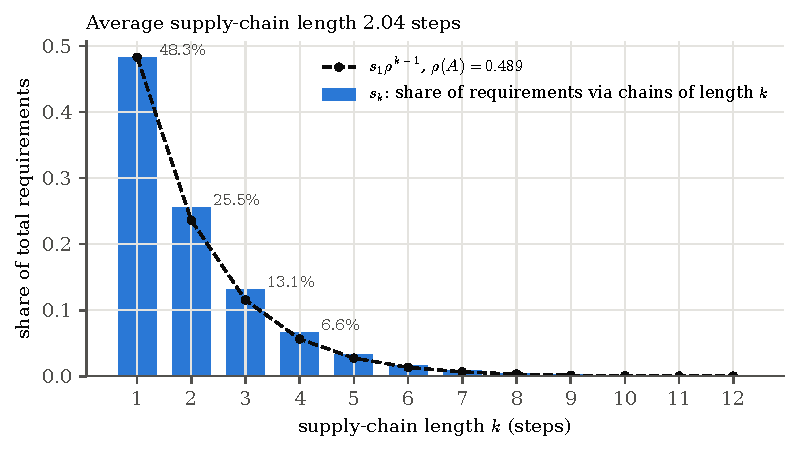
\includegraphics[width=0.85\linewidth]{figures/fig-walks.pdf}
\caption{Share $s_k$ of all requirements carried by supply chains of exactly
$k$ steps (bars), with the geometric decay $s_1\rho(A)^{k-1}$ (dashed), for
the \NInd{} industries in 2017. Computation on the BEA tables of
Section~\ref{subsec:io-data}.}
\label{fig:walks}
\end{figure}

% ---------------------------------------------------------------------
\subsection{From requirements to a graph}
\label{subsec:threshold}

To ask how \emph{structured} the network is, we turn $A$ into a simple graph
of the kind studied in this article.

\begin{definition}[Threshold graph]
\label{def:threshold}
Let $w_{ij}=\max(a_{ij},a_{ji})$ for $i\ne j$. For $\theta>0$, the
\emph{threshold graph} $G_\theta$ has vertex set $\{1,\dots,N\}$, with $i\ne j$
adjacent if and only if $w_{ij}\ge\theta$, that is, if one of the two
industries buys at least $\theta$ dollars from the other per dollar of its own
output. Its adjacency matrix is $A_\theta$.
\end{definition}

Lowering $\theta$ adds edges and never removes them. No threshold is
privileged, so the two measures defined in Section~\ref{subsec:delta}, $\delta$
and $\bar\lambda-\bar\mu$, are reported over \NThetas{} thresholds spaced evenly
on a logarithmic scale from $10^{-4}$ (a hundredth of a cent per dollar) to
$10^{-1}$ (ten cents per dollar). The other quantities are reported at the
threshold at which $G_\theta$ has the density of $H(2,20)$, defined in
Section~\ref{subsec:benchmarks}.

% ---------------------------------------------------------------------
\subsection{Measuring distance from strong regularity}
\label{subsec:delta}

Let $G$ be a graph on $n$ vertices with adjacency matrix $A$, and write
$\bar A=J-I-A$ for the adjacency matrix of its complement. (In this subsection
and the next, $A$ is a $0/1$ adjacency matrix.) By Theorem~\ref{thm:walks},
for $u\ne v$ the entry $(A^2)_{uv}$ is the number of common neighbours of $u$
and $v$; we write $c(u,v)=(A^2)_{uv}$. The diagonal entry $(A^2)_{uu}$ is the
degree $d(u)$. Recall from Section~\ref{sec:srg} that $G$, neither complete nor
edgeless, is strongly regular with parameters $(n,k,\lambda,\mu)$ exactly when
\begin{equation}\label{eq:srg-identity}
  A^2=kI+\lambda A+\mu\bar A .
\end{equation}
The three matrices $I$, $A$, $\bar A$ have disjoint supports: $I$ covers the
diagonal, $A$ the ordered adjacent pairs, $\bar A$ the ordered non-adjacent
pairs. Equation \eqref{eq:srg-identity} therefore says three things at once:
every diagonal entry of $A^2$ equals $k$, every entry on an edge equals
$\lambda$, and every entry on a non-edge equals $\mu$. For a general graph
these entries are not constant. They form three lists:
\begin{equation}\label{eq:three-lists}
  \mathcal D=\bigl(d(u)\bigr)_{u},\qquad
  \mathcal L=\bigl(c(u,v)\bigr)_{u\sim v},\qquad
  \mathcal M=\bigl(c(u,v)\bigr)_{u\not\sim v,\,u\ne v},
\end{equation}
indexed by vertices, ordered adjacent pairs, and ordered distinct non-adjacent
pairs respectively. If $G$ has $m$ edges and $\bar m$ non-edges, the lists have
lengths $n$, $2m$ and $2\bar m$. Write $\bar d,\bar\lambda,\bar\mu$ for their
means and $\Var$ for the population variance of a list.

\begin{proposition}\label{prop:residual}
Let $G$ have at least one edge and at least one non-edge. For real
$k,\lambda,\mu$ let $R(k,\lambda,\mu)=A^2-kI-\lambda A-\mu\bar A$. Then
\begin{equation}\label{eq:residual}
  \min_{k,\lambda,\mu\in\R}\fro{R(k,\lambda,\mu)}^2
  = n\Var(\mathcal D)+2m\Var(\mathcal L)+2\bar m\Var(\mathcal M),
\end{equation}
and the minimum is attained exactly at $(k,\lambda,\mu)=(\bar d,\bar\lambda,\bar\mu)$.
\end{proposition}

\begin{proof}
Because $I$, $A$ and $\bar A$ have disjoint supports that together cover every
entry, the squared Frobenius norm splits as
\[
  \fro{R}^2=\sum_{u}\bigl(d(u)-k\bigr)^2
  +\sum_{u\sim v}\bigl(c(u,v)-\lambda\bigr)^2
  +\sum_{u\not\sim v,\,u\ne v}\bigl(c(u,v)-\mu\bigr)^2 ,
\]
with the last two sums over ordered pairs. Each term involves only one of
$k,\lambda,\mu$, so each can be minimised separately. For a list
$x_1,\dots,x_\ell$ and real $a$,
$\sum_i(x_i-a)^2=\ell\Var(x)+\ell(\bar x-a)^2$, which is minimised exactly at
$a=\bar x$ with minimum $\ell\Var(x)$. Applying this to each list gives
\eqref{eq:residual}.
\end{proof}

\begin{definition}[Distance from strong regularity]
\label{def:delta}
For $G$ with at least one edge and one non-edge, set
\[
  \delta(G)=\frac{\min_{k,\lambda,\mu}\fro{R(k,\lambda,\mu)}}{\fro{A^2}} .
\]
\end{definition}

Taking $k=\lambda=\mu=0$ gives $R=A^2$, so $0\le\delta(G)\le1$. The
normalisation makes $\delta$ comparable across thresholds, where the number of
edges changes.

\begin{corollary}\label{cor:delta-zero}
Let $G$ be neither complete nor edgeless. Then $\delta(G)=0$ if and only if
$G$ is strongly regular, in which case $(\bar d,\bar\lambda,\bar\mu)$ are its
parameters $(k,\lambda,\mu)$.
\end{corollary}

\begin{proof}
By Proposition~\ref{prop:residual}, $\delta(G)=0$ if and only if all three
lists in \eqref{eq:three-lists} are constant, which is \eqref{eq:srg-identity}
with $(k,\lambda,\mu)=(\bar d,\bar\lambda,\bar\mu)$.
\end{proof}

The degree term in \eqref{eq:residual} cannot be dropped: constant $\lambda$
and constant $\mu$ do not by themselves force a graph to be regular.

\begin{example}[The bow-tie]
\label{ex:bowtie}
Let $G$ be two triangles sharing one vertex, with vertices ordered
$v_0,v_1,v_2,v_3,v_4$, where $v_0$ is the shared vertex and the triangles are
$\{v_0,v_1,v_2\}$ and $\{v_0,v_3,v_4\}$. Then
\[
  A=\begin{pmatrix}
  0&1&1&1&1\\ 1&0&1&0&0\\ 1&1&0&0&0\\ 1&0&0&0&1\\ 1&0&0&1&0
  \end{pmatrix},
  \qquad
  A^2=\begin{pmatrix}
  4&1&1&1&1\\ 1&2&1&1&1\\ 1&1&2&1&1\\ 1&1&1&2&1\\ 1&1&1&1&2
  \end{pmatrix}.
\]
Every off-diagonal entry of $A^2$ is $1$, so $\mathcal L$ and $\mathcal M$ are
constant with $\lambda=\mu=1$. The degrees are $4,2,2,2,2$, so
$\bar d=12/5$, $\Var(\mathcal D)=32/5-(12/5)^2=16/25$, and by
\eqref{eq:residual} the minimum squared residual is $5\cdot16/25=16/5$.
The graph is not strongly regular, and only the degree term detects it.
By the friendship theorem of Erd\H{o}s, R\'enyi and S\'os
\cite{erdos1966friendship}, the finite graphs in which every two distinct
vertices have exactly one common neighbour are precisely the graphs consisting
of triangles sharing a common vertex, so the bow-tie is the smallest graph
with $\lambda=\mu=1$ that is not regular. Other values give smaller examples:
the path $v_1v_2v_3$ has $\lambda=0$ and $\mu=1$, with degrees $1,2,1$.
\end{example}

% ---------------------------------------------------------------------
\subsection{The benchmarks}
\label{subsec:benchmarks}

\paragraph{Random graphs.} The random graph $G(n,p)$ of Gilbert
\cite{gilbert1959}, usually called the Erd\H{o}s--R\'enyi model, includes each
of the $\binom n2$ possible edges independently with probability $p$. Erd\H{o}s
and R\'enyi \cite{erdos1959} studied the closely related model with a fixed
number of edges.

\begin{proposition}\label{prop:er}
In $G(n,p)$, each degree $d(u)$ has distribution $\Bin(n-1,p)$. For distinct
$u,v$, the count $c(u,v)$ has distribution $\Bin(n-2,p^2)$ and is independent
of whether $u$ and $v$ are adjacent.
\end{proposition}

\begin{proof}
The degree of $u$ counts which of the $n-1$ independent edges at $u$ are
present. For $u\ne v$, a third vertex $w$ is a common neighbour exactly when
both $uw$ and $vw$ are edges, which has probability $p^2$; these events for the
$n-2$ choices of $w$ involve disjoint pairs of edges and so are independent.
None of them involves the edge $uv$, so $c(u,v)$ is independent of it.
\end{proof}

So in a random graph, adjacency tells us nothing about common neighbours:
$\mathcal L$ and $\mathcal M$ have the same distribution, and
$\bar\lambda-\bar\mu$ is close to zero.

\paragraph{Graphs with the same degrees.} A random graph differs from
$G_\theta$ in two ways at once: its degrees are nearly equal, and its edges
are placed independently. To separate the two, we also compare with random
graphs that have \emph{exactly} the degree sequence of $G_\theta$, generated by
repeated double-edge swaps \cite{maslov2002}: two edges $\{a,b\}$ and $\{c,d\}$
are replaced by $\{a,d\}$ and $\{c,b\}$ whenever this creates no loop or
repeated edge, which leaves every degree unchanged. We make five swap attempts
per edge. This benchmark is a computation; we prove nothing about it.

For each $\theta$ we report the mean and the central $95\%$ range of $\delta$
and of $\bar\lambda-\bar\mu$ over \NER{} Erd\H{o}s--R\'enyi graphs with the
density of $G_\theta$, and over \NDP{} degree-preserving rewirings of
$G_\theta$ (\NDPStar{} at $\theta^\ast$ below). These ranges are computations,
not theorems.

\paragraph{A strongly regular graph.} By Corollary~\ref{cor:delta-zero}, every
strongly regular graph has $\delta=0$. For the spectral comparison we want a
specific strongly regular graph of the same order. Choosing $N=400$ makes one
available from Section~\ref{sec:johnson-hamming}: the Hamming graph $H(2,20)$
\cite[Example~2.2.2]{mentorthesis}, whose vertices are the pairs $(a,b)$ with
$a,b\in\{0,\dots,19\}$, adjacent when they differ in exactly one coordinate.
Its parameters are
$(n,k,\lambda,\mu)=(400,38,18,2)$, its non-trivial eigenvalues are the roots of
$x^2-(\lambda-\mu)x+(\mu-k)=x^2-16x-36$ \cite{brouwer2012}, namely $18$ and $-2$, with
multiplicities $38$ and $361$ (one checks $38+38\cdot18-361\cdot2=0=\tr A$),
and its largest cliques are its $40$ ``lines'' of $20$ vertices. We write
$\theta^\ast$ for the threshold at which $G_\theta$ has exactly the density of
$H(2,20)$, hence mean degree $38$; on our data
$\theta^\ast=\ThetaStar$, that is, \ThetaStarCents{} cents per dollar.

% ---------------------------------------------------------------------
\subsection{Results}
\label{subsec:supply-results}

All numbers and figures in this subsection are computations on the 2017 BEA
tables, except where another year is named. Figure~\ref{fig:adjacency} shows
the adjacency matrix of $G_{\theta^\ast}$, first in the ordering by industry
code used throughout and then with the industries grouped by sector. The two
matrices are $A_{\theta^\ast}$ and $PA_{\theta^\ast}P^{\mathsf T}$ for a
permutation matrix $P$, so they describe the same graph.

\begin{figure}[htbp]
\centering
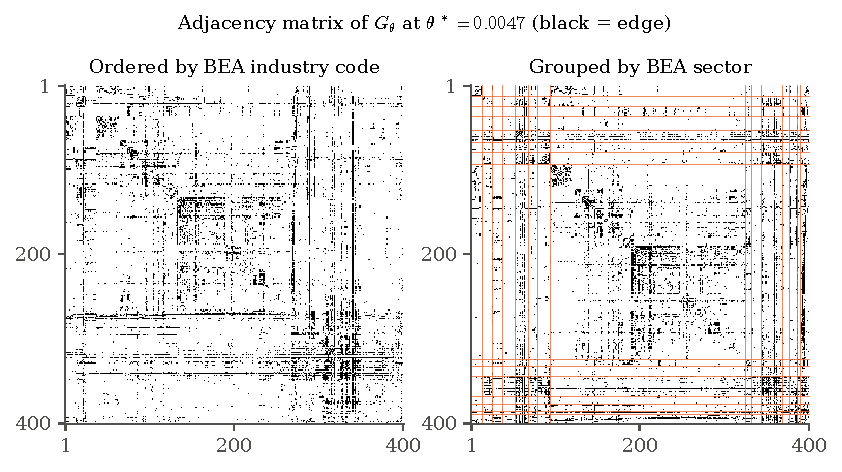
\includegraphics[width=0.9\linewidth]{figures/fig-adjacency.pdf}
\caption{The adjacency matrix of $G_{\theta^\ast}$, $\theta^\ast=\ThetaStar$,
with industries in order of BEA code (left) and grouped by BEA sector
(right; lines mark sector boundaries). Black entries are $1$. The dense rows
and columns are the hub industries, which trade with most other
industries.}
\label{fig:adjacency}
\end{figure}

\paragraph{The graph at $\theta^\ast$.} $G_{\theta^\ast}$ has \EdgesStar{}
edges and mean degree \MeanDegStar, but its degrees are very unequal: their
standard deviation is \SdDegStar, against \ERSdDeg{} for a random graph of the
same density, and the largest is \MaxDegStar. The highest degrees belong to
industries that trade with most other industries: \HubOne{}
(\HubOneDeg), \HubTwo{} (\HubTwoDeg), \HubThree{} (\HubThreeDeg) and \HubFour{}
(\HubFourDeg). They appear as the dense rows and columns in
Figure~\ref{fig:adjacency}. The graph has \ComponentsStar{} components; the
\IsolatedStar{} isolated vertices are BEA's ``customs duties'' and ``private
households'' industries, which have no intermediate inputs. Its clique number
is \CliqueStar. Edges are only mildly concentrated inside the fifteen BEA
sectors: \FracWithinSector\% of edges lie inside a sector, against
\FracWithinSectorExp\% of all pairs of industries.

\paragraph{Common neighbours.} Figure~\ref{fig:common-neighbours} applies the
instrument of Section~\ref{subsec:delta} to $G_{\theta^\ast}$. In the random
graph, $\mathcal L$ and $\mathcal M$ have the same distribution, as
Proposition~\ref{prop:er} requires, with mean $(N-2)p^2=\ERCommon$. In the
industry network they separate: adjacent pairs have on average
$\bar\lambda=\LambdaFitStar$ common neighbours and non-adjacent pairs
$\bar\mu=\MuFitStar$, a gap of $\bar\lambda-\bar\mu=\GapStar$. The gap lies in
$[\ERGapLoStar,\ERGapHiStar]$ for random graphs of this density and in
$[\DPGapLoStar,\DPGapHiStar]$ for graphs with the network's own degrees; for
$H(2,20)$ it is $\lambda-\mu=16$. So adjacency predicts shared trading
partners far better than in a random graph, and somewhat better than the
unequal degrees alone would produce, but less sharply than in the strongly
regular benchmark. Figure~\ref{fig:delta-sweep}(b) shows that the order holds
at every threshold: the gap exceeds both random ranges for every $\theta$ in
\RangeGapAboveDP.

\begin{figure}[htbp]
\centering
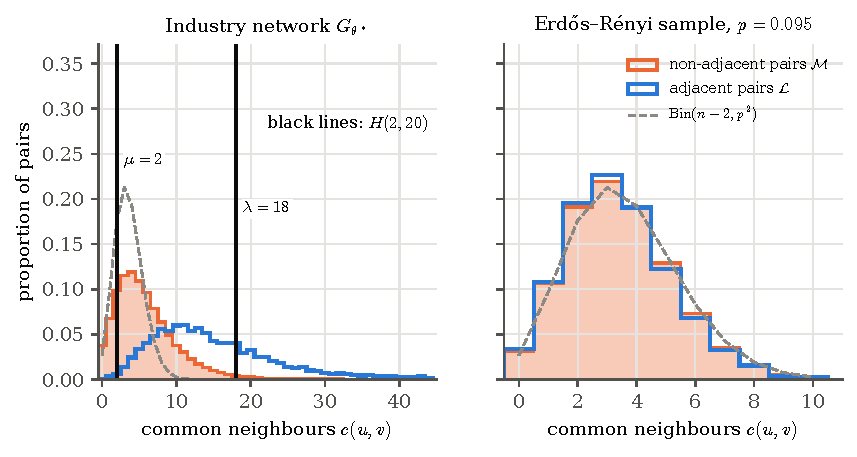
\includegraphics[width=0.95\linewidth]{figures/fig-common-neighbours.pdf}
\caption{Distributions of the common-neighbour counts $c(u,v)$ for adjacent
pairs ($\mathcal L$, blue) and non-adjacent pairs ($\mathcal M$, orange), in
$G_{\theta^\ast}$ (left) and in one Erd\H{o}s--R\'enyi graph of the same
density (right), with the distribution $\Bin(N-2,p^2)$ that
Proposition~\ref{prop:er} predicts for both lists in the random graph
(dashed). Black lines: the constant values $\lambda=18$ and $\mu=2$ of
$H(2,20)$.}
\label{fig:common-neighbours}
\end{figure}

\paragraph{Distance from strong regularity.} At $\theta^\ast$,
$\delta(G_{\theta^\ast})=\DeltaStar$. By Proposition~\ref{prop:residual} the
squared residual splits into three parts: \FracEdgeStar\% from the spread of
$\mathcal L$ (standard deviation \SdLambdaStar), \FracNonedgeStar\% from the
spread of $\mathcal M$ (standard deviation \SdMuStar), and only
\FracDegreeStar\% from the unequal degrees, large as they are. Random graphs of
the same density give $\delta$ in $[\ERDeltaLoStar,\ERDeltaHiStar]$, and
graphs with the same degrees give $[\DPDeltaLoStar,\DPDeltaHiStar]$. The
industry network is therefore further from strong regularity than a random
graph of its density, but slightly closer than a random graph with its
degrees. Figure~\ref{fig:delta-sweep}(a) shows the same order across the
sweep: $\delta(G_\theta)$ lies above the random-graph range for every $\theta$
in \RangeDeltaAboveER{} and below the degree-preserving range for every
$\theta$ in \RangeDeltaBelowDP.

\begin{figure}[htbp]
\centering
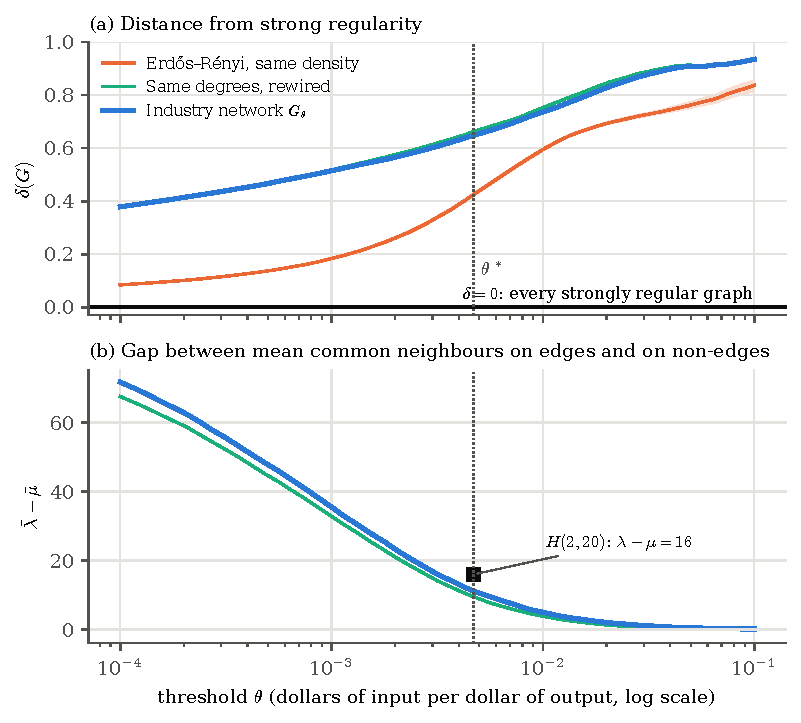
\includegraphics[width=0.9\linewidth]{figures/fig-delta-sweep.pdf}
\caption{(a) Distance from strong regularity $\delta(G_\theta)$ as the
threshold varies, for the industry network (blue), random graphs of the same
density (orange) and random graphs with the same degree sequence (green);
shading is the central $95\%$ range of the benchmarks. The line $\delta=0$ is
every strongly regular graph. (b) The gap $\bar\lambda-\bar\mu$ for the same
graphs, and $\lambda-\mu=16$ for $H(2,20)$. The dotted line marks
$\theta^\ast$. The horizontal axis is logarithmic.}
\label{fig:delta-sweep}
\end{figure}

\paragraph{Spectra.} Figure~\ref{fig:spectra} compares the adjacency spectra
at $\theta^\ast$. $H(2,20)$ has three distinct eigenvalues; the industry
network has \DistinctStar{} (to within $10^{-6}$) and the random graph
\ERDistinct, so on this count the industry network is as far from strong
regularity as a random graph. Its largest eigenvalue is \LambdaOneAStar,
against \ERLambdaOne{} for the random graph: a largest eigenvalue well above
the mean degree $38$ is what very unequal degrees produce, since it lies
between the mean and the maximum degree (Section~\ref{sec:spectra}).

\begin{figure}[htbp]
\centering
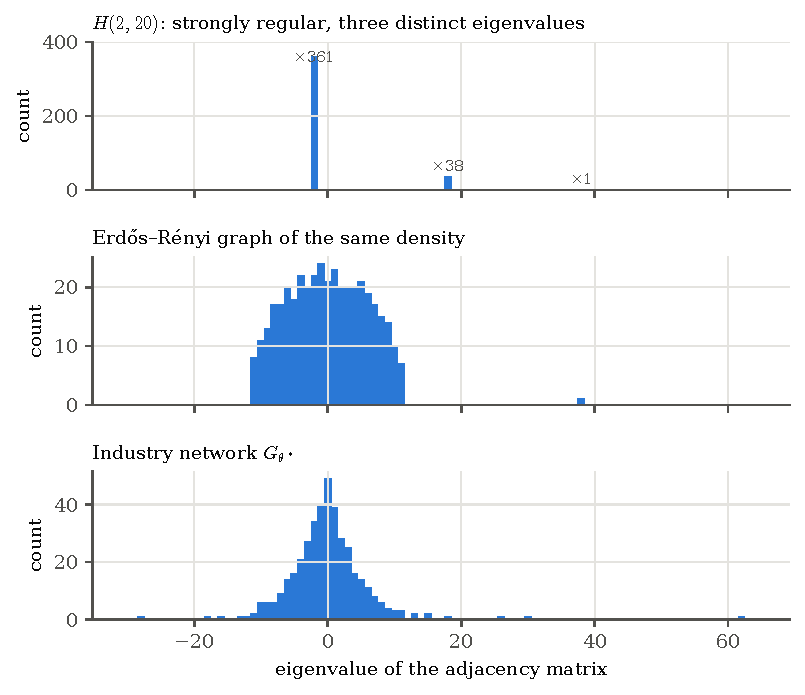
\includegraphics[width=0.85\linewidth]{figures/fig-spectra.pdf}
\caption{Adjacency spectra of $H(2,20)$ (three distinct eigenvalues, with
multiplicities), of one Erd\H{o}s--R\'enyi graph of the same density as
$G_{\theta^\ast}$, and of $G_{\theta^\ast}$.}
\label{fig:spectra}
\end{figure}

\begin{table}[htbp]
\centering
\small
\caption{The three graphs at $\theta^\ast=\ThetaStar$. The $H(2,20)$ column is
exact and $G_{\theta^\ast}$ is a computation on the 2017 tables. In the
Erd\H{o}s--R\'enyi column: (a) expected value, by construction; (b) one
sample; (c) the expectation $(N-2)p^2$ from Proposition~\ref{prop:er};
(d) mean over \NER{} samples.}
\label{tab:supply-summary}
\begin{tabular}{@{}lccc@{}}
\toprule
 & $H(2,20)$ & Erd\H{o}s--R\'enyi & $G_{\theta^\ast}$ \\
\midrule
Mean degree $\bar d$                 & $38$  & $38^{a}$             & $\MeanDegStar$ \\
Standard deviation of degree         & $0$   & $\ERSdDeg^{b}$       & $\SdDegStar$ \\
$\bar\lambda$                        & $18$  & $\ERCommon^{c}$      & $\LambdaFitStar$ \\
$\bar\mu$                            & $2$   & $\ERCommon^{c}$      & $\MuFitStar$ \\
$\bar\lambda-\bar\mu$                & $16$  & $\ERGapStar^{d}$     & $\GapStar$ \\
$\delta$                             & $0$   & $\ERDeltaStar^{d}$   & $\DeltaStar$ \\
Distinct eigenvalues of $A$          & $3$   & $\ERDistinct^{b}$    & $\DistinctStar$ \\
Largest eigenvalue of $A$            & $38$  & $\ERLambdaOne^{b}$   & $\LambdaOneAStar$ \\
Clique number                        & $20$  & $\ERClique^{b}$      & $\CliqueStar$ \\
\bottomrule
\end{tabular}
\end{table}

\paragraph{Stability over time.} The same analysis on the 2012 tables, at the
same level of detail, gives $\theta^\ast=\ThetaStarTwelve$, a gap
$\bar\lambda-\bar\mu=\GapTwelve$ (degree-preserving upper end \DPGapHiTwelve)
and $\delta=\DeltaTwelve$ (random-graph upper end \ERDeltaHiTwelve,
degree-preserving lower end \DPDeltaLoTwelve), the same pattern as in 2017.
At the coarser level of \NSummary{} industries, available for every year from
\YearFirst{} to \YearLast, we repeat the analysis at the threshold that matches
the density of $H(2,20)$ (Figure~\ref{fig:years}). In all \NYears{} years the
gap exceeds the degree-preserving range and $\delta$ lies between the two
random ranges. Across the years $\rho(A)$ stays between \YearsRhoMin{}
(\YearsRhoMinYear) and \YearsRhoMax{} (\YearsRhoMaxYear), and the average
supply-chain length between \YearsAPLMin{} and \YearsAPLMax{} steps.

\begin{figure}[htbp]
\centering
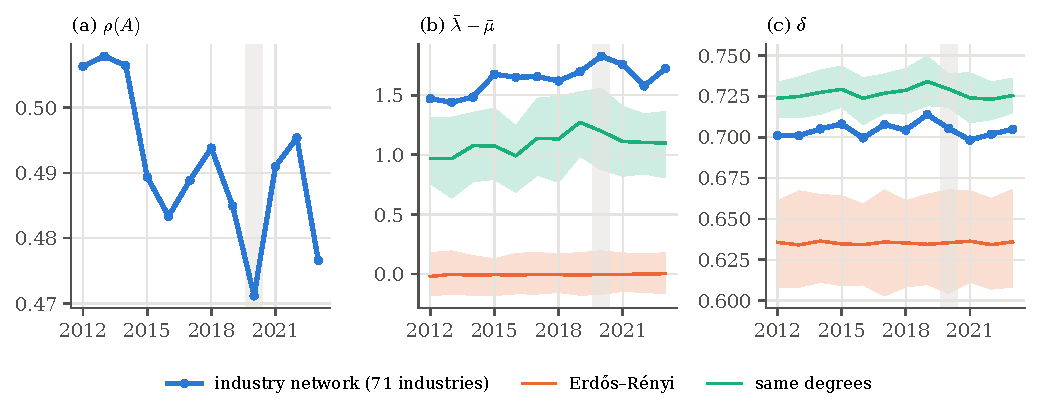
\includegraphics[width=\linewidth]{figures/fig-years.pdf}
\caption{Year by year, \YearFirst--\YearLast, for the \NSummary{}-industry
tables: (a) the spectral radius $\rho(A)$; (b) the gap $\bar\lambda-\bar\mu$
and (c) $\delta$, at the threshold matching the density of $H(2,20)$, with the
central $95\%$ ranges of the two random benchmarks. The year 2020 is shaded.}
\label{fig:years}
\end{figure}

\paragraph{Summary.} On these tables, supply chains are short: half of all
requirements are direct purchases, and the average chain is about two steps
long, with longer chains decaying at the rate $\rho(A)$. As a graph, the
network is dominated by a few service industries that supply most other
industries.
Even so, whether two industries trade directly predicts how many trading
partners they share more strongly than the unequal degrees alone would
produce. What separates the network from strong regularity is variation: the
number of shared partners varies greatly from one pair to the next, which
accounts for most of $\delta$. These are statements about the US input--output
tables over 2012--2023, not general facts about supply chains.

% ---------------------------------------------------------------------
\subsection{Limitations}
\label{subsec:supply-limits}

An industry aggregates many firms, so an edge between two industries does not
mean that any particular firms trade; firm-level supplier networks are not
publicly available. The tables record total requirements, including inputs
that were imported, so $A$ describes the technology of US production rather
than purely domestic supply chains. Thresholding discards both the size of
each requirement and its direction; we report a sweep of thresholds for the
first reason, and the directed matrix $A$ itself is used in
Section~\ref{subsec:walks}. Restricting to the $400$ largest industries treats
the two smallest as outside suppliers; no industry buys more than
\DroppedShare{} cents of inputs from them per dollar of its output. Finally, the benchmarks are deliberately extreme: a
network that sits between them is neither perfectly uniform nor random, which
is informative but is not a model of how supply chains form.
      % where the section goes
%  Requires amsmath, amssymb, amsthm, graphicx, booktabs, and the theorem
%  environments definition, theorem, proposition, corollary, remark, example.
%
%  Every number below is a macro from generated/numbers.tex, written by
%  scripts/run_analysis.py. Do not type numbers into this file by hand:
%  rerun the pipeline instead, and the text stays consistent with the code.
% =====================================================================

\providecommand{\R}{\mathbb{R}}
\providecommand{\tr}{\operatorname{tr}}
\providecommand{\Var}{\operatorname{Var}}
\providecommand{\Bin}{\operatorname{Bin}}
\providecommand{\fro}[1]{\lVert #1\rVert_F}
\providecommand{\1}{\mathbf{1}}

\section{An application: supply chains in the US economy}
\label{sec:supply}

Every industry buys inputs from other industries, which buy inputs from others
in turn. The resulting network of supply chains is recorded, for the whole US
economy, in the input--output accounts of the Bureau of Economic Analysis, and
it is the standard object for studying how a disruption in one industry
travels to others \cite{acemoglu2012,carvalho2014}. This
section applies the article's machinery to that network in two ways. First, the
theorem that powers of an adjacency matrix count walks (Theorem~\ref{thm:walks})
has a weighted form, and in that form it \emph{is} the standard description of
how requirements travel along supply chains. Second, the definition of strong
regularity becomes a measuring instrument: we build a graph from the network and
measure how far it is from strongly regular, using random graphs and a strongly
regular graph as benchmarks. Strongly regular graphs do not occur in economic
data, and nothing here claims that they do.

Table~\ref{tab:supply-status} records how strong each connection is, so that a
reader can tell a theorem from a modelling choice.

\begin{table}[htbp]
\centering
\small
\caption{Strength of each link between the article's mathematics and the
supply-chain application.}
\label{tab:supply-status}
\begin{tabular}{@{}p{0.44\linewidth}p{0.17\linewidth}p{0.31\linewidth}@{}}
\toprule
Connection & Status & Support \\
\midrule
Powers of $A$ count weighted supply chains & Direct & Theorem~\ref{thm:weighted-walks} (proved here) \\
Total requirements $=\sum_k A^k$ & Direct & Theorem~\ref{thm:neumann} (proved here) \\
Average supply-chain length & Direct & Proposition~\ref{prop:chain-length} (proved here) \\
$(A_\theta^2)_{uv}$ counts common neighbours & Direct & Theorem~\ref{thm:walks} \\
Distance from strong regularity, $\delta(G)$ & Direct & Proposition~\ref{prop:residual} (proved here) \\
Erd\H{o}s--R\'enyi graph as a null model & Benchmark & Proposition~\ref{prop:er} (proved here) \\
Graphs with the same degree sequence & Benchmark & Computation \\
Strongly regular graph $H(2,20)$ & Benchmark & Corollary~\ref{cor:delta-zero} \\
Industries as stand-ins for firms & Approximation & Industries aggregate many firms \\
\bottomrule
\end{tabular}
\end{table}

% ---------------------------------------------------------------------
\subsection{The data: requirements between industries}
\label{subsec:io-data}

The Bureau of Economic Analysis records, for each year, how much of each
commodity every industry buys (the \emph{Use} table) and how much of each
commodity every industry produces (the \emph{Make} table), in millions of
dollars \cite{horowitz2009}. We use the tables at producer prices, before
redefinitions, in the 2017 industry classification, as redistributed
in the U.S. Environmental Protection Agency's open-source package
\texttt{useeior} \cite{li2022useeior,bea2025io}. From them we form the
standard industry-by-industry matrix \cite[Ch.~5]{miller2009}.

\begin{definition}[Direct requirements]
\label{def:direct}
Let $U$ be the commodity-by-industry matrix of intermediate purchases, $V$ the
industry-by-commodity matrix of production, $g=V\1$ the vector of industry
outputs and $q=V^{\mathsf T}\1$ the vector of commodity outputs. Every
industry has $g_j>0$; let $B=U\,\mathrm{diag}(g)^{-1}$, and let $D$ have
entries $d_{ic}=v_{ic}/q_c$, with $d_{ic}=0$ when $q_c=0$ (a few commodities,
such as used goods, are produced by no industry). The
\emph{direct-requirements matrix} is $A=DB$. Its entry $a_{ij}\ge 0$ is the
number of dollars of industry $i$'s output used directly to produce one dollar
of industry $j$'s output.
\end{definition}

Column $j$ of $A$ is industry $j$'s recipe of intermediate inputs per dollar
of output; the rest of each dollar pays for labour, capital, taxes and imports
not produced by any US industry. We take the $N=\NInd$ industries with the
largest gross output in 2017, out of \NIndSource, numbered $1,\dots,N$ in
order of their BEA industry code; this ordering is used for every matrix in
this section. We work mainly with 2017, and repeat the analysis for 2012 at
this level and for every year from \YearFirst{} to \YearLast{} at the coarser
level of \NSummary{} industries. In each Use table a handful of entries are
negative (in the 2017 detail table, for example, entries for used and
secondhand goods and for a few farm and food products); we set them to zero,
so that $A$ is entrywise non-negative. All
computations in this section are on these public tables and are labelled as
such. The code that produces every number, table and figure is publicly
available.\footnote{\url{https://github.com/desaidaksh1206-netizen/supply-chain-graphs-srg}}

% ---------------------------------------------------------------------
\subsection{Supply chains are weighted walks}
\label{subsec:walks}

Regard $A$ as a weighted adjacency matrix of a directed graph on the
industries, with an arc $i\to j$ of weight $a_{ij}$ whenever $a_{ij}>0$: an arc
points from a supplier to a buyer. A \emph{supply chain of length $k$} from $i$
to $j$ is a walk $i=v_0\to v_1\to\dots\to v_k=j$, and its \emph{weight} is the
product $a_{v_0v_1}a_{v_1v_2}\cdots a_{v_{k-1}v_k}$.

\begin{theorem}[Weighted walks]
\label{thm:weighted-walks}
For every $k\ge1$, $(A^k)_{ij}$ is the sum of the weights of all walks of
length $k$ from $i$ to $j$.
\end{theorem}

\begin{proof}
For $k=1$ the only walk of length one from $i$ to $j$ is the arc itself, of
weight $a_{ij}$. Suppose the statement holds for $k$. Every walk of length
$k+1$ from $i$ to $j$ is a walk of length $k$ from $i$ to some vertex $\ell$,
followed by the arc $\ell\to j$, and its weight is the product of the two
weights. Summing over $\ell$ and using the induction hypothesis,
$\sum_\ell (A^k)_{i\ell}\,a_{\ell j}=(A^{k+1})_{ij}$.
\end{proof}

With all weights equal to $1$ this is Theorem~\ref{thm:walks}. The weighted
form has a direct reading: to make one dollar of $j$'s output, industry $j$
uses $a_{\ell j}$ dollars from each supplier $\ell$, each of which uses
$a_{i\ell}$ dollars of $i$'s output per dollar, and so on back along the chain.
So $(A^k)_{ij}$ is the amount of $i$'s output, in dollars, that one dollar of
$j$'s output requires through chains with exactly $k-1$ intermediate
industries.

\begin{theorem}[Total requirements]
\label{thm:neumann}
Let $A\ge0$ have spectral radius $\rho(A)<1$. Then $I-A$ is invertible,
\begin{equation}\label{eq:neumann}
  L=(I-A)^{-1}=I+A+A^2+A^3+\cdots,
\end{equation}
and every entry of $L$ is non-negative.
\end{theorem}

\begin{proof}
Because $\rho(A)<1$, $A^k\to0$ as $k\to\infty$ \cite[Sec.~5.6]{horn2013}.
For each $k$,
$(I-A)(I+A+\dots+A^k)=I-A^{k+1}$. If $(I-A)x=0$ then $x=A^{k+1}x\to0$, so
$x=0$ and $I-A$ is invertible. Multiplying by $(I-A)^{-1}$ gives
$I+A+\dots+A^k=(I-A)^{-1}(I-A^{k+1})\to(I-A)^{-1}$. Every partial sum is
non-negative, so the limit is.
\end{proof}

$L$ is the Leontief inverse \cite{leontief1936}. By
Theorem~\ref{thm:weighted-walks}, $L_{ij}$ adds up the requirements of one
dollar of $j$'s output for $i$'s output along supply chains of every length.
Its column sums are the \emph{output multipliers}: the total output, across
the economy, needed to deliver one dollar of $j$'s product to final users
\cite[Ch.~6]{miller2009}.

The hypothesis $\rho(A)<1$ is often checked through the following bound.

\begin{proposition}\label{prop:colsum}
For any real square matrix, $\rho(A)\le\max_j\sum_i|a_{ij}|$.
\end{proposition}

\begin{proof}
Let $Av=\lambda v$ with $v\ne0$, and write $\|x\|_1=\sum_i|x_i|$. Then
\[
  |\lambda|\,\|v\|_1=\|Av\|_1\le\sum_j|v_j|\sum_i|a_{ij}|
  \le\Bigl(\max_j\sum_i|a_{ij}|\Bigr)\|v\|_1 ,
\]
and dividing by $\|v\|_1>0$ gives the bound for every eigenvalue.
\end{proof}

Since column $j$ of $A$ sums to the share of $j$'s output spent on
intermediate inputs, one expects every column sum to be below $1$. On our data
that fails for exactly \NColAboveOne{} industry, state and local government
passenger transit: its value added is negative in the tables, and its
intermediate purchases are \MaxColSum{} times the value of its output.
Proposition~\ref{prop:colsum} therefore does not apply. We compute $\rho(A)$ directly instead:
$\rho(A)=\Rho$ for 2017 and \RhoTwelve{} for 2012, so
Theorem~\ref{thm:neumann} holds. The partial sum $I+A+\dots+A^{20}$ of
\eqref{eq:neumann} is within $\NeumannTwenty$ of $L$, entry by entry.

\begin{proposition}[Average supply-chain length]
\label{prop:chain-length}
Let $A\ge0$ with $\rho(A)<1$ and $A\ne0$, and let
$s_k=\1^{\mathsf T}A^k\1\big/\1^{\mathsf T}(L-I)\1$ for $k\ge1$. Then
$\sum_{k\ge1}s_k=1$ and
\[
  \sum_{k\ge1}k\,s_k=\frac{\1^{\mathsf T}(L-I)L\,\1}{\1^{\mathsf T}(L-I)\1}.
\]
\end{proposition}

\begin{proof}
By \eqref{eq:neumann}, $L-I=\sum_{k\ge1}A^k$, which gives the first claim.
By Gelfand's formula $\rho(A)=\lim_{k\to\infty}\lVert A^k\rVert^{1/k}$
\cite[Sec.~5.6]{horn2013}, for any $r$ with $\rho(A)<r<1$ there is a constant
$C$ with $\lVert A^k\rVert\le Cr^k$ for all $k$, so $\sum_{k\ge1}kA^{k}$
converges absolutely. Its terms are non-negative, so it can be rearranged:
$\sum_{k\ge1}kA^k=\sum_{k\ge1}\sum_{j\ge k}A^j=\sum_{k\ge1}A^k L=(L-I)L$,
since $\sum_{j\ge k}A^j=A^kL$.
\end{proof}

So $s_k$ is the share of all requirements, direct and indirect, that travels
along chains of exactly $k$ steps, and $\sum_k k s_k$ is the average length of
a supply chain weighted by the dollars it carries; it is an economy-wide
version of the average propagation length of \cite{dietzenbacher2005}.

Figure~\ref{fig:walks} shows the result (computation). Direct purchases carry
$s_1=\ShareOne\%$ of all requirements, two-step chains $\ShareTwo\%$, three-step
chains $\ShareThree\%$, and chains of four or more steps the remaining
$\ShareBeyondThree\%$. The average supply-chain length is \APL{} steps
(\APLTwelve{} in 2012). Successive shares shrink by a nearly constant factor:
$s_{k+1}/s_k$ lies between \RatioMin{} and \RatioMax{} for $k=1,\dots,8$,
close to $\rho(A)=\Rho$. This is what one expects: by Perron--Frobenius
theory, $\rho(A)$ is itself an eigenvalue of the non-negative matrix $A$, with
a non-negative eigenvector \cite[Sec.~8.3]{horn2013}, and the largest
eigenvalue sets the rate at which $A^k$ decays. Output
multipliers range from \MultMin{} to \MultMax, with mean \MultMean: on average,
delivering a dollar of final product requires about two dollars of output across
the economy.

\begin{figure}[htbp]
\centering
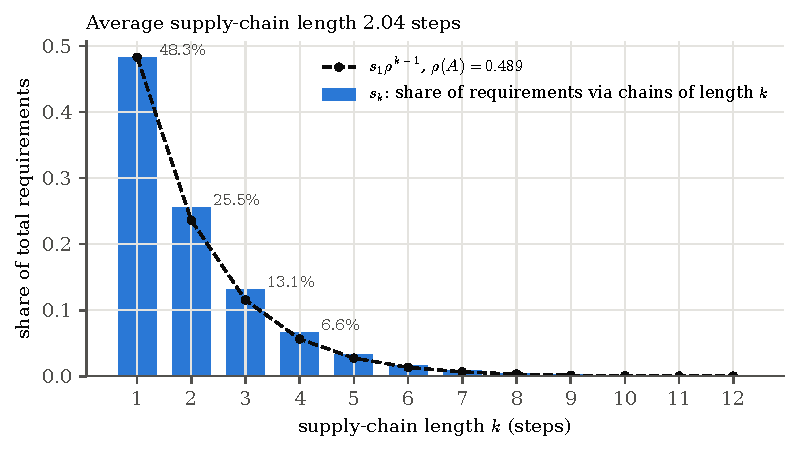
\includegraphics[width=0.85\linewidth]{figures/fig-walks.pdf}
\caption{Share $s_k$ of all requirements carried by supply chains of exactly
$k$ steps (bars), with the geometric decay $s_1\rho(A)^{k-1}$ (dashed), for
the \NInd{} industries in 2017. Computation on the BEA tables of
Section~\ref{subsec:io-data}.}
\label{fig:walks}
\end{figure}

% ---------------------------------------------------------------------
\subsection{From requirements to a graph}
\label{subsec:threshold}

To ask how \emph{structured} the network is, we turn $A$ into a simple graph
of the kind studied in this article.

\begin{definition}[Threshold graph]
\label{def:threshold}
Let $w_{ij}=\max(a_{ij},a_{ji})$ for $i\ne j$. For $\theta>0$, the
\emph{threshold graph} $G_\theta$ has vertex set $\{1,\dots,N\}$, with $i\ne j$
adjacent if and only if $w_{ij}\ge\theta$, that is, if one of the two
industries buys at least $\theta$ dollars from the other per dollar of its own
output. Its adjacency matrix is $A_\theta$.
\end{definition}

Lowering $\theta$ adds edges and never removes them. No threshold is
privileged, so the two measures defined in Section~\ref{subsec:delta}, $\delta$
and $\bar\lambda-\bar\mu$, are reported over \NThetas{} thresholds spaced evenly
on a logarithmic scale from $10^{-4}$ (a hundredth of a cent per dollar) to
$10^{-1}$ (ten cents per dollar). The other quantities are reported at the
threshold at which $G_\theta$ has the density of $H(2,20)$, defined in
Section~\ref{subsec:benchmarks}.

% ---------------------------------------------------------------------
\subsection{Measuring distance from strong regularity}
\label{subsec:delta}

Let $G$ be a graph on $n$ vertices with adjacency matrix $A$, and write
$\bar A=J-I-A$ for the adjacency matrix of its complement. (In this subsection
and the next, $A$ is a $0/1$ adjacency matrix.) By Theorem~\ref{thm:walks},
for $u\ne v$ the entry $(A^2)_{uv}$ is the number of common neighbours of $u$
and $v$; we write $c(u,v)=(A^2)_{uv}$. The diagonal entry $(A^2)_{uu}$ is the
degree $d(u)$. Recall from Section~\ref{sec:srg} that $G$, neither complete nor
edgeless, is strongly regular with parameters $(n,k,\lambda,\mu)$ exactly when
\begin{equation}\label{eq:srg-identity}
  A^2=kI+\lambda A+\mu\bar A .
\end{equation}
The three matrices $I$, $A$, $\bar A$ have disjoint supports: $I$ covers the
diagonal, $A$ the ordered adjacent pairs, $\bar A$ the ordered non-adjacent
pairs. Equation \eqref{eq:srg-identity} therefore says three things at once:
every diagonal entry of $A^2$ equals $k$, every entry on an edge equals
$\lambda$, and every entry on a non-edge equals $\mu$. For a general graph
these entries are not constant. They form three lists:
\begin{equation}\label{eq:three-lists}
  \mathcal D=\bigl(d(u)\bigr)_{u},\qquad
  \mathcal L=\bigl(c(u,v)\bigr)_{u\sim v},\qquad
  \mathcal M=\bigl(c(u,v)\bigr)_{u\not\sim v,\,u\ne v},
\end{equation}
indexed by vertices, ordered adjacent pairs, and ordered distinct non-adjacent
pairs respectively. If $G$ has $m$ edges and $\bar m$ non-edges, the lists have
lengths $n$, $2m$ and $2\bar m$. Write $\bar d,\bar\lambda,\bar\mu$ for their
means and $\Var$ for the population variance of a list.

\begin{proposition}\label{prop:residual}
Let $G$ have at least one edge and at least one non-edge. For real
$k,\lambda,\mu$ let $R(k,\lambda,\mu)=A^2-kI-\lambda A-\mu\bar A$. Then
\begin{equation}\label{eq:residual}
  \min_{k,\lambda,\mu\in\R}\fro{R(k,\lambda,\mu)}^2
  = n\Var(\mathcal D)+2m\Var(\mathcal L)+2\bar m\Var(\mathcal M),
\end{equation}
and the minimum is attained exactly at $(k,\lambda,\mu)=(\bar d,\bar\lambda,\bar\mu)$.
\end{proposition}

\begin{proof}
Because $I$, $A$ and $\bar A$ have disjoint supports that together cover every
entry, the squared Frobenius norm splits as
\[
  \fro{R}^2=\sum_{u}\bigl(d(u)-k\bigr)^2
  +\sum_{u\sim v}\bigl(c(u,v)-\lambda\bigr)^2
  +\sum_{u\not\sim v,\,u\ne v}\bigl(c(u,v)-\mu\bigr)^2 ,
\]
with the last two sums over ordered pairs. Each term involves only one of
$k,\lambda,\mu$, so each can be minimised separately. For a list
$x_1,\dots,x_\ell$ and real $a$,
$\sum_i(x_i-a)^2=\ell\Var(x)+\ell(\bar x-a)^2$, which is minimised exactly at
$a=\bar x$ with minimum $\ell\Var(x)$. Applying this to each list gives
\eqref{eq:residual}.
\end{proof}

\begin{definition}[Distance from strong regularity]
\label{def:delta}
For $G$ with at least one edge and one non-edge, set
\[
  \delta(G)=\frac{\min_{k,\lambda,\mu}\fro{R(k,\lambda,\mu)}}{\fro{A^2}} .
\]
\end{definition}

Taking $k=\lambda=\mu=0$ gives $R=A^2$, so $0\le\delta(G)\le1$. The
normalisation makes $\delta$ comparable across thresholds, where the number of
edges changes.

\begin{corollary}\label{cor:delta-zero}
Let $G$ be neither complete nor edgeless. Then $\delta(G)=0$ if and only if
$G$ is strongly regular, in which case $(\bar d,\bar\lambda,\bar\mu)$ are its
parameters $(k,\lambda,\mu)$.
\end{corollary}

\begin{proof}
By Proposition~\ref{prop:residual}, $\delta(G)=0$ if and only if all three
lists in \eqref{eq:three-lists} are constant, which is \eqref{eq:srg-identity}
with $(k,\lambda,\mu)=(\bar d,\bar\lambda,\bar\mu)$.
\end{proof}

The degree term in \eqref{eq:residual} cannot be dropped: constant $\lambda$
and constant $\mu$ do not by themselves force a graph to be regular.

\begin{example}[The bow-tie]
\label{ex:bowtie}
Let $G$ be two triangles sharing one vertex, with vertices ordered
$v_0,v_1,v_2,v_3,v_4$, where $v_0$ is the shared vertex and the triangles are
$\{v_0,v_1,v_2\}$ and $\{v_0,v_3,v_4\}$. Then
\[
  A=\begin{pmatrix}
  0&1&1&1&1\\ 1&0&1&0&0\\ 1&1&0&0&0\\ 1&0&0&0&1\\ 1&0&0&1&0
  \end{pmatrix},
  \qquad
  A^2=\begin{pmatrix}
  4&1&1&1&1\\ 1&2&1&1&1\\ 1&1&2&1&1\\ 1&1&1&2&1\\ 1&1&1&1&2
  \end{pmatrix}.
\]
Every off-diagonal entry of $A^2$ is $1$, so $\mathcal L$ and $\mathcal M$ are
constant with $\lambda=\mu=1$. The degrees are $4,2,2,2,2$, so
$\bar d=12/5$, $\Var(\mathcal D)=32/5-(12/5)^2=16/25$, and by
\eqref{eq:residual} the minimum squared residual is $5\cdot16/25=16/5$.
The graph is not strongly regular, and only the degree term detects it.
By the friendship theorem of Erd\H{o}s, R\'enyi and S\'os
\cite{erdos1966friendship}, the finite graphs in which every two distinct
vertices have exactly one common neighbour are precisely the graphs consisting
of triangles sharing a common vertex, so the bow-tie is the smallest graph
with $\lambda=\mu=1$ that is not regular. Other values give smaller examples:
the path $v_1v_2v_3$ has $\lambda=0$ and $\mu=1$, with degrees $1,2,1$.
\end{example}

% ---------------------------------------------------------------------
\subsection{The benchmarks}
\label{subsec:benchmarks}

\paragraph{Random graphs.} The random graph $G(n,p)$ of Gilbert
\cite{gilbert1959}, usually called the Erd\H{o}s--R\'enyi model, includes each
of the $\binom n2$ possible edges independently with probability $p$. Erd\H{o}s
and R\'enyi \cite{erdos1959} studied the closely related model with a fixed
number of edges.

\begin{proposition}\label{prop:er}
In $G(n,p)$, each degree $d(u)$ has distribution $\Bin(n-1,p)$. For distinct
$u,v$, the count $c(u,v)$ has distribution $\Bin(n-2,p^2)$ and is independent
of whether $u$ and $v$ are adjacent.
\end{proposition}

\begin{proof}
The degree of $u$ counts which of the $n-1$ independent edges at $u$ are
present. For $u\ne v$, a third vertex $w$ is a common neighbour exactly when
both $uw$ and $vw$ are edges, which has probability $p^2$; these events for the
$n-2$ choices of $w$ involve disjoint pairs of edges and so are independent.
None of them involves the edge $uv$, so $c(u,v)$ is independent of it.
\end{proof}

So in a random graph, adjacency tells us nothing about common neighbours:
$\mathcal L$ and $\mathcal M$ have the same distribution, and
$\bar\lambda-\bar\mu$ is close to zero.

\paragraph{Graphs with the same degrees.} A random graph differs from
$G_\theta$ in two ways at once: its degrees are nearly equal, and its edges
are placed independently. To separate the two, we also compare with random
graphs that have \emph{exactly} the degree sequence of $G_\theta$, generated by
repeated double-edge swaps \cite{maslov2002}: two edges $\{a,b\}$ and $\{c,d\}$
are replaced by $\{a,d\}$ and $\{c,b\}$ whenever this creates no loop or
repeated edge, which leaves every degree unchanged. We make five swap attempts
per edge. This benchmark is a computation; we prove nothing about it.

For each $\theta$ we report the mean and the central $95\%$ range of $\delta$
and of $\bar\lambda-\bar\mu$ over \NER{} Erd\H{o}s--R\'enyi graphs with the
density of $G_\theta$, and over \NDP{} degree-preserving rewirings of
$G_\theta$ (\NDPStar{} at $\theta^\ast$ below). These ranges are computations,
not theorems.

\paragraph{A strongly regular graph.} By Corollary~\ref{cor:delta-zero}, every
strongly regular graph has $\delta=0$. For the spectral comparison we want a
specific strongly regular graph of the same order. Choosing $N=400$ makes one
available from Section~\ref{sec:johnson-hamming}: the Hamming graph $H(2,20)$
\cite[Example~2.2.2]{mentorthesis}, whose vertices are the pairs $(a,b)$ with
$a,b\in\{0,\dots,19\}$, adjacent when they differ in exactly one coordinate.
Its parameters are
$(n,k,\lambda,\mu)=(400,38,18,2)$, its non-trivial eigenvalues are the roots of
$x^2-(\lambda-\mu)x+(\mu-k)=x^2-16x-36$ \cite{brouwer2012}, namely $18$ and $-2$, with
multiplicities $38$ and $361$ (one checks $38+38\cdot18-361\cdot2=0=\tr A$),
and its largest cliques are its $40$ ``lines'' of $20$ vertices. We write
$\theta^\ast$ for the threshold at which $G_\theta$ has exactly the density of
$H(2,20)$, hence mean degree $38$; on our data
$\theta^\ast=\ThetaStar$, that is, \ThetaStarCents{} cents per dollar.

% ---------------------------------------------------------------------
\subsection{Results}
\label{subsec:supply-results}

All numbers and figures in this subsection are computations on the 2017 BEA
tables, except where another year is named. Figure~\ref{fig:adjacency} shows
the adjacency matrix of $G_{\theta^\ast}$, first in the ordering by industry
code used throughout and then with the industries grouped by sector. The two
matrices are $A_{\theta^\ast}$ and $PA_{\theta^\ast}P^{\mathsf T}$ for a
permutation matrix $P$, so they describe the same graph.

\begin{figure}[htbp]
\centering
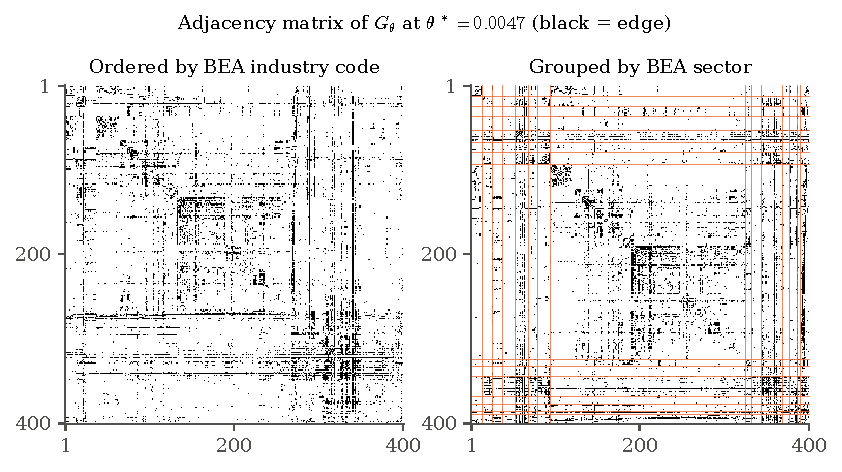
\includegraphics[width=0.9\linewidth]{figures/fig-adjacency.pdf}
\caption{The adjacency matrix of $G_{\theta^\ast}$, $\theta^\ast=\ThetaStar$,
with industries in order of BEA code (left) and grouped by BEA sector
(right; lines mark sector boundaries). Black entries are $1$. The dense rows
and columns are the hub industries, which trade with most other
industries.}
\label{fig:adjacency}
\end{figure}

\paragraph{The graph at $\theta^\ast$.} $G_{\theta^\ast}$ has \EdgesStar{}
edges and mean degree \MeanDegStar, but its degrees are very unequal: their
standard deviation is \SdDegStar, against \ERSdDeg{} for a random graph of the
same density, and the largest is \MaxDegStar. The highest degrees belong to
industries that trade with most other industries: \HubOne{}
(\HubOneDeg), \HubTwo{} (\HubTwoDeg), \HubThree{} (\HubThreeDeg) and \HubFour{}
(\HubFourDeg). They appear as the dense rows and columns in
Figure~\ref{fig:adjacency}. The graph has \ComponentsStar{} components; the
\IsolatedStar{} isolated vertices are BEA's ``customs duties'' and ``private
households'' industries, which have no intermediate inputs. Its clique number
is \CliqueStar. Edges are only mildly concentrated inside the fifteen BEA
sectors: \FracWithinSector\% of edges lie inside a sector, against
\FracWithinSectorExp\% of all pairs of industries.

\paragraph{Common neighbours.} Figure~\ref{fig:common-neighbours} applies the
instrument of Section~\ref{subsec:delta} to $G_{\theta^\ast}$. In the random
graph, $\mathcal L$ and $\mathcal M$ have the same distribution, as
Proposition~\ref{prop:er} requires, with mean $(N-2)p^2=\ERCommon$. In the
industry network they separate: adjacent pairs have on average
$\bar\lambda=\LambdaFitStar$ common neighbours and non-adjacent pairs
$\bar\mu=\MuFitStar$, a gap of $\bar\lambda-\bar\mu=\GapStar$. The gap lies in
$[\ERGapLoStar,\ERGapHiStar]$ for random graphs of this density and in
$[\DPGapLoStar,\DPGapHiStar]$ for graphs with the network's own degrees; for
$H(2,20)$ it is $\lambda-\mu=16$. So adjacency predicts shared trading
partners far better than in a random graph, and somewhat better than the
unequal degrees alone would produce, but less sharply than in the strongly
regular benchmark. Figure~\ref{fig:delta-sweep}(b) shows that the order holds
at every threshold: the gap exceeds both random ranges for every $\theta$ in
\RangeGapAboveDP.

\begin{figure}[htbp]
\centering
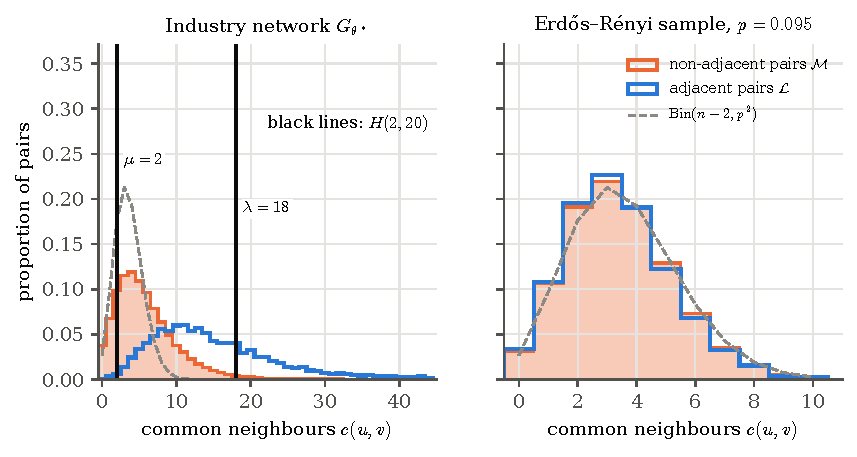
\includegraphics[width=0.95\linewidth]{figures/fig-common-neighbours.pdf}
\caption{Distributions of the common-neighbour counts $c(u,v)$ for adjacent
pairs ($\mathcal L$, blue) and non-adjacent pairs ($\mathcal M$, orange), in
$G_{\theta^\ast}$ (left) and in one Erd\H{o}s--R\'enyi graph of the same
density (right), with the distribution $\Bin(N-2,p^2)$ that
Proposition~\ref{prop:er} predicts for both lists in the random graph
(dashed). Black lines: the constant values $\lambda=18$ and $\mu=2$ of
$H(2,20)$.}
\label{fig:common-neighbours}
\end{figure}

\paragraph{Distance from strong regularity.} At $\theta^\ast$,
$\delta(G_{\theta^\ast})=\DeltaStar$. By Proposition~\ref{prop:residual} the
squared residual splits into three parts: \FracEdgeStar\% from the spread of
$\mathcal L$ (standard deviation \SdLambdaStar), \FracNonedgeStar\% from the
spread of $\mathcal M$ (standard deviation \SdMuStar), and only
\FracDegreeStar\% from the unequal degrees, large as they are. Random graphs of
the same density give $\delta$ in $[\ERDeltaLoStar,\ERDeltaHiStar]$, and
graphs with the same degrees give $[\DPDeltaLoStar,\DPDeltaHiStar]$. The
industry network is therefore further from strong regularity than a random
graph of its density, but slightly closer than a random graph with its
degrees. Figure~\ref{fig:delta-sweep}(a) shows the same order across the
sweep: $\delta(G_\theta)$ lies above the random-graph range for every $\theta$
in \RangeDeltaAboveER{} and below the degree-preserving range for every
$\theta$ in \RangeDeltaBelowDP.

\begin{figure}[htbp]
\centering
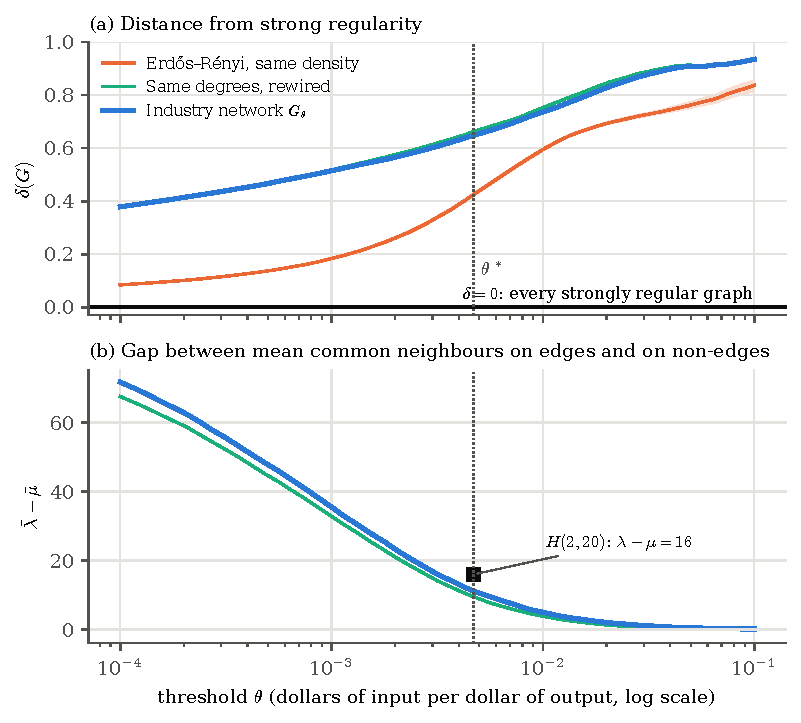
\includegraphics[width=0.9\linewidth]{figures/fig-delta-sweep.pdf}
\caption{(a) Distance from strong regularity $\delta(G_\theta)$ as the
threshold varies, for the industry network (blue), random graphs of the same
density (orange) and random graphs with the same degree sequence (green);
shading is the central $95\%$ range of the benchmarks. The line $\delta=0$ is
every strongly regular graph. (b) The gap $\bar\lambda-\bar\mu$ for the same
graphs, and $\lambda-\mu=16$ for $H(2,20)$. The dotted line marks
$\theta^\ast$. The horizontal axis is logarithmic.}
\label{fig:delta-sweep}
\end{figure}

\paragraph{Spectra.} Figure~\ref{fig:spectra} compares the adjacency spectra
at $\theta^\ast$. $H(2,20)$ has three distinct eigenvalues; the industry
network has \DistinctStar{} (to within $10^{-6}$) and the random graph
\ERDistinct, so on this count the industry network is as far from strong
regularity as a random graph. Its largest eigenvalue is \LambdaOneAStar,
against \ERLambdaOne{} for the random graph: a largest eigenvalue well above
the mean degree $38$ is what very unequal degrees produce, since it lies
between the mean and the maximum degree (Section~\ref{sec:spectra}).

\begin{figure}[htbp]
\centering
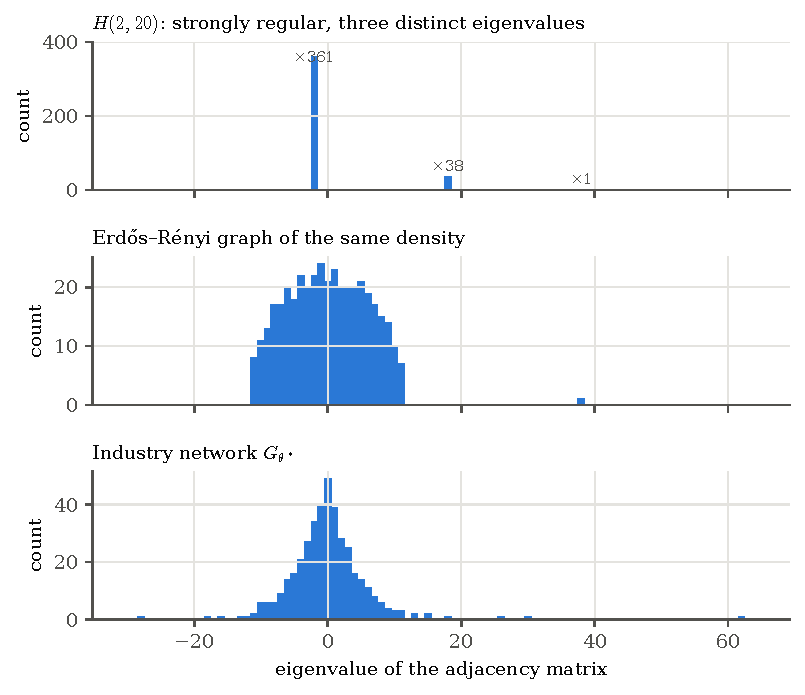
\includegraphics[width=0.85\linewidth]{figures/fig-spectra.pdf}
\caption{Adjacency spectra of $H(2,20)$ (three distinct eigenvalues, with
multiplicities), of one Erd\H{o}s--R\'enyi graph of the same density as
$G_{\theta^\ast}$, and of $G_{\theta^\ast}$.}
\label{fig:spectra}
\end{figure}

\begin{table}[htbp]
\centering
\small
\caption{The three graphs at $\theta^\ast=\ThetaStar$. The $H(2,20)$ column is
exact and $G_{\theta^\ast}$ is a computation on the 2017 tables. In the
Erd\H{o}s--R\'enyi column: (a) expected value, by construction; (b) one
sample; (c) the expectation $(N-2)p^2$ from Proposition~\ref{prop:er};
(d) mean over \NER{} samples.}
\label{tab:supply-summary}
\begin{tabular}{@{}lccc@{}}
\toprule
 & $H(2,20)$ & Erd\H{o}s--R\'enyi & $G_{\theta^\ast}$ \\
\midrule
Mean degree $\bar d$                 & $38$  & $38^{a}$             & $\MeanDegStar$ \\
Standard deviation of degree         & $0$   & $\ERSdDeg^{b}$       & $\SdDegStar$ \\
$\bar\lambda$                        & $18$  & $\ERCommon^{c}$      & $\LambdaFitStar$ \\
$\bar\mu$                            & $2$   & $\ERCommon^{c}$      & $\MuFitStar$ \\
$\bar\lambda-\bar\mu$                & $16$  & $\ERGapStar^{d}$     & $\GapStar$ \\
$\delta$                             & $0$   & $\ERDeltaStar^{d}$   & $\DeltaStar$ \\
Distinct eigenvalues of $A$          & $3$   & $\ERDistinct^{b}$    & $\DistinctStar$ \\
Largest eigenvalue of $A$            & $38$  & $\ERLambdaOne^{b}$   & $\LambdaOneAStar$ \\
Clique number                        & $20$  & $\ERClique^{b}$      & $\CliqueStar$ \\
\bottomrule
\end{tabular}
\end{table}

\paragraph{Stability over time.} The same analysis on the 2012 tables, at the
same level of detail, gives $\theta^\ast=\ThetaStarTwelve$, a gap
$\bar\lambda-\bar\mu=\GapTwelve$ (degree-preserving upper end \DPGapHiTwelve)
and $\delta=\DeltaTwelve$ (random-graph upper end \ERDeltaHiTwelve,
degree-preserving lower end \DPDeltaLoTwelve), the same pattern as in 2017.
At the coarser level of \NSummary{} industries, available for every year from
\YearFirst{} to \YearLast, we repeat the analysis at the threshold that matches
the density of $H(2,20)$ (Figure~\ref{fig:years}). In all \NYears{} years the
gap exceeds the degree-preserving range and $\delta$ lies between the two
random ranges. Across the years $\rho(A)$ stays between \YearsRhoMin{}
(\YearsRhoMinYear) and \YearsRhoMax{} (\YearsRhoMaxYear), and the average
supply-chain length between \YearsAPLMin{} and \YearsAPLMax{} steps.

\begin{figure}[htbp]
\centering
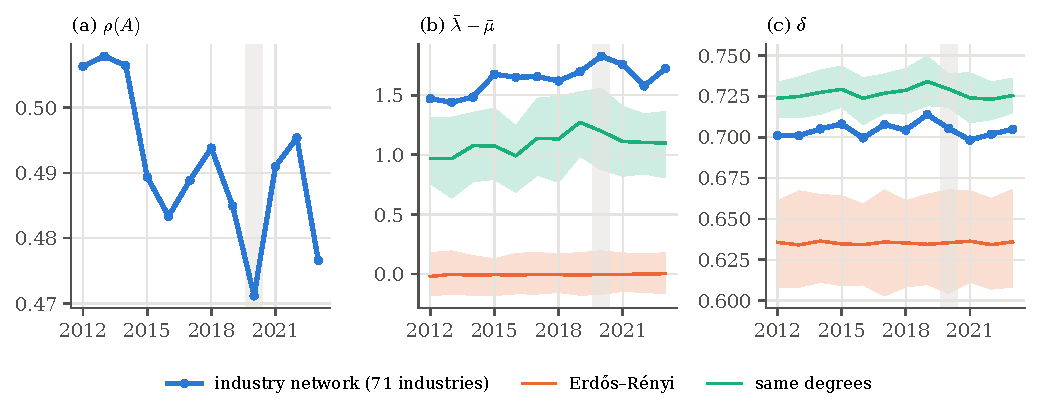
\includegraphics[width=\linewidth]{figures/fig-years.pdf}
\caption{Year by year, \YearFirst--\YearLast, for the \NSummary{}-industry
tables: (a) the spectral radius $\rho(A)$; (b) the gap $\bar\lambda-\bar\mu$
and (c) $\delta$, at the threshold matching the density of $H(2,20)$, with the
central $95\%$ ranges of the two random benchmarks. The year 2020 is shaded.}
\label{fig:years}
\end{figure}

\paragraph{Summary.} On these tables, supply chains are short: half of all
requirements are direct purchases, and the average chain is about two steps
long, with longer chains decaying at the rate $\rho(A)$. As a graph, the
network is dominated by a few service industries that supply most other
industries.
Even so, whether two industries trade directly predicts how many trading
partners they share more strongly than the unequal degrees alone would
produce. What separates the network from strong regularity is variation: the
number of shared partners varies greatly from one pair to the next, which
accounts for most of $\delta$. These are statements about the US input--output
tables over 2012--2023, not general facts about supply chains.

% ---------------------------------------------------------------------
\subsection{Limitations}
\label{subsec:supply-limits}

An industry aggregates many firms, so an edge between two industries does not
mean that any particular firms trade; firm-level supplier networks are not
publicly available. The tables record total requirements, including inputs
that were imported, so $A$ describes the technology of US production rather
than purely domestic supply chains. Thresholding discards both the size of
each requirement and its direction; we report a sweep of thresholds for the
first reason, and the directed matrix $A$ itself is used in
Section~\ref{subsec:walks}. Restricting to the $400$ largest industries treats
the two smallest as outside suppliers; no industry buys more than
\DroppedShare{} cents of inputs from them per dollar of its output. Finally, the benchmarks are deliberately extreme: a
network that sits between them is neither perfectly uniform nor random, which
is informative but is not a model of how supply chains form.
      % where the section goes
%  Requires amsmath, amssymb, amsthm, graphicx, booktabs, and the theorem
%  environments definition, theorem, proposition, corollary, remark, example.
%
%  Every number below is a macro from generated/numbers.tex, written by
%  scripts/run_analysis.py. Do not type numbers into this file by hand:
%  rerun the pipeline instead, and the text stays consistent with the code.
% =====================================================================

\providecommand{\R}{\mathbb{R}}
\providecommand{\tr}{\operatorname{tr}}
\providecommand{\Var}{\operatorname{Var}}
\providecommand{\Bin}{\operatorname{Bin}}
\providecommand{\fro}[1]{\lVert #1\rVert_F}
\providecommand{\1}{\mathbf{1}}

\section{An application: supply chains in the US economy}
\label{sec:supply}

Every industry buys inputs from other industries, which buy inputs from others
in turn. The resulting network of supply chains is recorded, for the whole US
economy, in the input--output accounts of the Bureau of Economic Analysis, and
it is the standard object for studying how a disruption in one industry
travels to others \cite{acemoglu2012,carvalho2014}. This
section applies the article's machinery to that network in two ways. First, the
theorem that powers of an adjacency matrix count walks (Theorem~\ref{thm:walks})
has a weighted form, and in that form it \emph{is} the standard description of
how requirements travel along supply chains. Second, the definition of strong
regularity becomes a measuring instrument: we build a graph from the network and
measure how far it is from strongly regular, using random graphs and a strongly
regular graph as benchmarks. Strongly regular graphs do not occur in economic
data, and nothing here claims that they do.

Table~\ref{tab:supply-status} records how strong each connection is, so that a
reader can tell a theorem from a modelling choice.

\begin{table}[htbp]
\centering
\small
\caption{Strength of each link between the article's mathematics and the
supply-chain application.}
\label{tab:supply-status}
\begin{tabular}{@{}p{0.44\linewidth}p{0.17\linewidth}p{0.31\linewidth}@{}}
\toprule
Connection & Status & Support \\
\midrule
Powers of $A$ count weighted supply chains & Direct & Theorem~\ref{thm:weighted-walks} (proved here) \\
Total requirements $=\sum_k A^k$ & Direct & Theorem~\ref{thm:neumann} (proved here) \\
Average supply-chain length & Direct & Proposition~\ref{prop:chain-length} (proved here) \\
$(A_\theta^2)_{uv}$ counts common neighbours & Direct & Theorem~\ref{thm:walks} \\
Distance from strong regularity, $\delta(G)$ & Direct & Proposition~\ref{prop:residual} (proved here) \\
Erd\H{o}s--R\'enyi graph as a null model & Benchmark & Proposition~\ref{prop:er} (proved here) \\
Graphs with the same degree sequence & Benchmark & Computation \\
Strongly regular graph $H(2,20)$ & Benchmark & Corollary~\ref{cor:delta-zero} \\
Industries as stand-ins for firms & Approximation & Industries aggregate many firms \\
\bottomrule
\end{tabular}
\end{table}

% ---------------------------------------------------------------------
\subsection{The data: requirements between industries}
\label{subsec:io-data}

The Bureau of Economic Analysis records, for each year, how much of each
commodity every industry buys (the \emph{Use} table) and how much of each
commodity every industry produces (the \emph{Make} table), in millions of
dollars \cite{horowitz2009}. We use the tables at producer prices, before
redefinitions, in the 2017 industry classification, as redistributed
in the U.S. Environmental Protection Agency's open-source package
\texttt{useeior} \cite{li2022useeior,bea2025io}. From them we form the
standard industry-by-industry matrix \cite[Ch.~5]{miller2009}.

\begin{definition}[Direct requirements]
\label{def:direct}
Let $U$ be the commodity-by-industry matrix of intermediate purchases, $V$ the
industry-by-commodity matrix of production, $g=V\1$ the vector of industry
outputs and $q=V^{\mathsf T}\1$ the vector of commodity outputs. Every
industry has $g_j>0$; let $B=U\,\mathrm{diag}(g)^{-1}$, and let $D$ have
entries $d_{ic}=v_{ic}/q_c$, with $d_{ic}=0$ when $q_c=0$ (a few commodities,
such as used goods, are produced by no industry). The
\emph{direct-requirements matrix} is $A=DB$. Its entry $a_{ij}\ge 0$ is the
number of dollars of industry $i$'s output used directly to produce one dollar
of industry $j$'s output.
\end{definition}

Column $j$ of $A$ is industry $j$'s recipe of intermediate inputs per dollar
of output; the rest of each dollar pays for labour, capital, taxes and imports
not produced by any US industry. We take the $N=\NInd$ industries with the
largest gross output in 2017, out of \NIndSource, numbered $1,\dots,N$ in
order of their BEA industry code; this ordering is used for every matrix in
this section. We work mainly with 2017, and repeat the analysis for 2012 at
this level and for every year from \YearFirst{} to \YearLast{} at the coarser
level of \NSummary{} industries. In each Use table a handful of entries are
negative (in the 2017 detail table, for example, entries for used and
secondhand goods and for a few farm and food products); we set them to zero,
so that $A$ is entrywise non-negative. All
computations in this section are on these public tables and are labelled as
such. The code that produces every number, table and figure is publicly
available.\footnote{\url{https://github.com/desaidaksh1206-netizen/supply-chain-graphs-srg}}

% ---------------------------------------------------------------------
\subsection{Supply chains are weighted walks}
\label{subsec:walks}

Regard $A$ as a weighted adjacency matrix of a directed graph on the
industries, with an arc $i\to j$ of weight $a_{ij}$ whenever $a_{ij}>0$: an arc
points from a supplier to a buyer. A \emph{supply chain of length $k$} from $i$
to $j$ is a walk $i=v_0\to v_1\to\dots\to v_k=j$, and its \emph{weight} is the
product $a_{v_0v_1}a_{v_1v_2}\cdots a_{v_{k-1}v_k}$.

\begin{theorem}[Weighted walks]
\label{thm:weighted-walks}
For every $k\ge1$, $(A^k)_{ij}$ is the sum of the weights of all walks of
length $k$ from $i$ to $j$.
\end{theorem}

\begin{proof}
For $k=1$ the only walk of length one from $i$ to $j$ is the arc itself, of
weight $a_{ij}$. Suppose the statement holds for $k$. Every walk of length
$k+1$ from $i$ to $j$ is a walk of length $k$ from $i$ to some vertex $\ell$,
followed by the arc $\ell\to j$, and its weight is the product of the two
weights. Summing over $\ell$ and using the induction hypothesis,
$\sum_\ell (A^k)_{i\ell}\,a_{\ell j}=(A^{k+1})_{ij}$.
\end{proof}

With all weights equal to $1$ this is Theorem~\ref{thm:walks}. The weighted
form has a direct reading: to make one dollar of $j$'s output, industry $j$
uses $a_{\ell j}$ dollars from each supplier $\ell$, each of which uses
$a_{i\ell}$ dollars of $i$'s output per dollar, and so on back along the chain.
So $(A^k)_{ij}$ is the amount of $i$'s output, in dollars, that one dollar of
$j$'s output requires through chains with exactly $k-1$ intermediate
industries.

\begin{theorem}[Total requirements]
\label{thm:neumann}
Let $A\ge0$ have spectral radius $\rho(A)<1$. Then $I-A$ is invertible,
\begin{equation}\label{eq:neumann}
  L=(I-A)^{-1}=I+A+A^2+A^3+\cdots,
\end{equation}
and every entry of $L$ is non-negative.
\end{theorem}

\begin{proof}
Because $\rho(A)<1$, $A^k\to0$ as $k\to\infty$ \cite[Sec.~5.6]{horn2013}.
For each $k$,
$(I-A)(I+A+\dots+A^k)=I-A^{k+1}$. If $(I-A)x=0$ then $x=A^{k+1}x\to0$, so
$x=0$ and $I-A$ is invertible. Multiplying by $(I-A)^{-1}$ gives
$I+A+\dots+A^k=(I-A)^{-1}(I-A^{k+1})\to(I-A)^{-1}$. Every partial sum is
non-negative, so the limit is.
\end{proof}

$L$ is the Leontief inverse \cite{leontief1936}. By
Theorem~\ref{thm:weighted-walks}, $L_{ij}$ adds up the requirements of one
dollar of $j$'s output for $i$'s output along supply chains of every length.
Its column sums are the \emph{output multipliers}: the total output, across
the economy, needed to deliver one dollar of $j$'s product to final users
\cite[Ch.~6]{miller2009}.

The hypothesis $\rho(A)<1$ is often checked through the following bound.

\begin{proposition}\label{prop:colsum}
For any real square matrix, $\rho(A)\le\max_j\sum_i|a_{ij}|$.
\end{proposition}

\begin{proof}
Let $Av=\lambda v$ with $v\ne0$, and write $\|x\|_1=\sum_i|x_i|$. Then
\[
  |\lambda|\,\|v\|_1=\|Av\|_1\le\sum_j|v_j|\sum_i|a_{ij}|
  \le\Bigl(\max_j\sum_i|a_{ij}|\Bigr)\|v\|_1 ,
\]
and dividing by $\|v\|_1>0$ gives the bound for every eigenvalue.
\end{proof}

Since column $j$ of $A$ sums to the share of $j$'s output spent on
intermediate inputs, one expects every column sum to be below $1$. On our data
that fails for exactly \NColAboveOne{} industry, state and local government
passenger transit: its value added is negative in the tables, and its
intermediate purchases are \MaxColSum{} times the value of its output.
Proposition~\ref{prop:colsum} therefore does not apply. We compute $\rho(A)$ directly instead:
$\rho(A)=\Rho$ for 2017 and \RhoTwelve{} for 2012, so
Theorem~\ref{thm:neumann} holds. The partial sum $I+A+\dots+A^{20}$ of
\eqref{eq:neumann} is within $\NeumannTwenty$ of $L$, entry by entry.

\begin{proposition}[Average supply-chain length]
\label{prop:chain-length}
Let $A\ge0$ with $\rho(A)<1$ and $A\ne0$, and let
$s_k=\1^{\mathsf T}A^k\1\big/\1^{\mathsf T}(L-I)\1$ for $k\ge1$. Then
$\sum_{k\ge1}s_k=1$ and
\[
  \sum_{k\ge1}k\,s_k=\frac{\1^{\mathsf T}(L-I)L\,\1}{\1^{\mathsf T}(L-I)\1}.
\]
\end{proposition}

\begin{proof}
By \eqref{eq:neumann}, $L-I=\sum_{k\ge1}A^k$, which gives the first claim.
By Gelfand's formula $\rho(A)=\lim_{k\to\infty}\lVert A^k\rVert^{1/k}$
\cite[Sec.~5.6]{horn2013}, for any $r$ with $\rho(A)<r<1$ there is a constant
$C$ with $\lVert A^k\rVert\le Cr^k$ for all $k$, so $\sum_{k\ge1}kA^{k}$
converges absolutely. Its terms are non-negative, so it can be rearranged:
$\sum_{k\ge1}kA^k=\sum_{k\ge1}\sum_{j\ge k}A^j=\sum_{k\ge1}A^k L=(L-I)L$,
since $\sum_{j\ge k}A^j=A^kL$.
\end{proof}

So $s_k$ is the share of all requirements, direct and indirect, that travels
along chains of exactly $k$ steps, and $\sum_k k s_k$ is the average length of
a supply chain weighted by the dollars it carries; it is an economy-wide
version of the average propagation length of \cite{dietzenbacher2005}.

Figure~\ref{fig:walks} shows the result (computation). Direct purchases carry
$s_1=\ShareOne\%$ of all requirements, two-step chains $\ShareTwo\%$, three-step
chains $\ShareThree\%$, and chains of four or more steps the remaining
$\ShareBeyondThree\%$. The average supply-chain length is \APL{} steps
(\APLTwelve{} in 2012). Successive shares shrink by a nearly constant factor:
$s_{k+1}/s_k$ lies between \RatioMin{} and \RatioMax{} for $k=1,\dots,8$,
close to $\rho(A)=\Rho$. This is what one expects: by Perron--Frobenius
theory, $\rho(A)$ is itself an eigenvalue of the non-negative matrix $A$, with
a non-negative eigenvector \cite[Sec.~8.3]{horn2013}, and the largest
eigenvalue sets the rate at which $A^k$ decays. Output
multipliers range from \MultMin{} to \MultMax, with mean \MultMean: on average,
delivering a dollar of final product requires about two dollars of output across
the economy.

\begin{figure}[htbp]
\centering
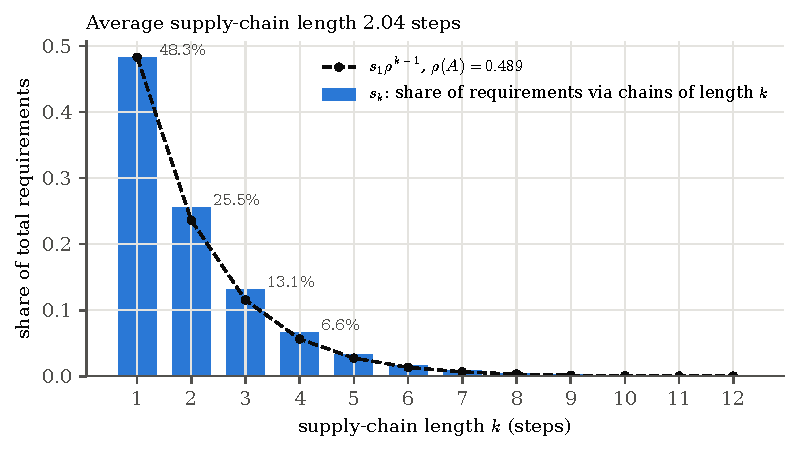
\includegraphics[width=0.85\linewidth]{figures/fig-walks.pdf}
\caption{Share $s_k$ of all requirements carried by supply chains of exactly
$k$ steps (bars), with the geometric decay $s_1\rho(A)^{k-1}$ (dashed), for
the \NInd{} industries in 2017. Computation on the BEA tables of
Section~\ref{subsec:io-data}.}
\label{fig:walks}
\end{figure}

% ---------------------------------------------------------------------
\subsection{From requirements to a graph}
\label{subsec:threshold}

To ask how \emph{structured} the network is, we turn $A$ into a simple graph
of the kind studied in this article.

\begin{definition}[Threshold graph]
\label{def:threshold}
Let $w_{ij}=\max(a_{ij},a_{ji})$ for $i\ne j$. For $\theta>0$, the
\emph{threshold graph} $G_\theta$ has vertex set $\{1,\dots,N\}$, with $i\ne j$
adjacent if and only if $w_{ij}\ge\theta$, that is, if one of the two
industries buys at least $\theta$ dollars from the other per dollar of its own
output. Its adjacency matrix is $A_\theta$.
\end{definition}

Lowering $\theta$ adds edges and never removes them. No threshold is
privileged, so the two measures defined in Section~\ref{subsec:delta}, $\delta$
and $\bar\lambda-\bar\mu$, are reported over \NThetas{} thresholds spaced evenly
on a logarithmic scale from $10^{-4}$ (a hundredth of a cent per dollar) to
$10^{-1}$ (ten cents per dollar). The other quantities are reported at the
threshold at which $G_\theta$ has the density of $H(2,20)$, defined in
Section~\ref{subsec:benchmarks}.

% ---------------------------------------------------------------------
\subsection{Measuring distance from strong regularity}
\label{subsec:delta}

Let $G$ be a graph on $n$ vertices with adjacency matrix $A$, and write
$\bar A=J-I-A$ for the adjacency matrix of its complement. (In this subsection
and the next, $A$ is a $0/1$ adjacency matrix.) By Theorem~\ref{thm:walks},
for $u\ne v$ the entry $(A^2)_{uv}$ is the number of common neighbours of $u$
and $v$; we write $c(u,v)=(A^2)_{uv}$. The diagonal entry $(A^2)_{uu}$ is the
degree $d(u)$. Recall from Section~\ref{sec:srg} that $G$, neither complete nor
edgeless, is strongly regular with parameters $(n,k,\lambda,\mu)$ exactly when
\begin{equation}\label{eq:srg-identity}
  A^2=kI+\lambda A+\mu\bar A .
\end{equation}
The three matrices $I$, $A$, $\bar A$ have disjoint supports: $I$ covers the
diagonal, $A$ the ordered adjacent pairs, $\bar A$ the ordered non-adjacent
pairs. Equation \eqref{eq:srg-identity} therefore says three things at once:
every diagonal entry of $A^2$ equals $k$, every entry on an edge equals
$\lambda$, and every entry on a non-edge equals $\mu$. For a general graph
these entries are not constant. They form three lists:
\begin{equation}\label{eq:three-lists}
  \mathcal D=\bigl(d(u)\bigr)_{u},\qquad
  \mathcal L=\bigl(c(u,v)\bigr)_{u\sim v},\qquad
  \mathcal M=\bigl(c(u,v)\bigr)_{u\not\sim v,\,u\ne v},
\end{equation}
indexed by vertices, ordered adjacent pairs, and ordered distinct non-adjacent
pairs respectively. If $G$ has $m$ edges and $\bar m$ non-edges, the lists have
lengths $n$, $2m$ and $2\bar m$. Write $\bar d,\bar\lambda,\bar\mu$ for their
means and $\Var$ for the population variance of a list.

\begin{proposition}\label{prop:residual}
Let $G$ have at least one edge and at least one non-edge. For real
$k,\lambda,\mu$ let $R(k,\lambda,\mu)=A^2-kI-\lambda A-\mu\bar A$. Then
\begin{equation}\label{eq:residual}
  \min_{k,\lambda,\mu\in\R}\fro{R(k,\lambda,\mu)}^2
  = n\Var(\mathcal D)+2m\Var(\mathcal L)+2\bar m\Var(\mathcal M),
\end{equation}
and the minimum is attained exactly at $(k,\lambda,\mu)=(\bar d,\bar\lambda,\bar\mu)$.
\end{proposition}

\begin{proof}
Because $I$, $A$ and $\bar A$ have disjoint supports that together cover every
entry, the squared Frobenius norm splits as
\[
  \fro{R}^2=\sum_{u}\bigl(d(u)-k\bigr)^2
  +\sum_{u\sim v}\bigl(c(u,v)-\lambda\bigr)^2
  +\sum_{u\not\sim v,\,u\ne v}\bigl(c(u,v)-\mu\bigr)^2 ,
\]
with the last two sums over ordered pairs. Each term involves only one of
$k,\lambda,\mu$, so each can be minimised separately. For a list
$x_1,\dots,x_\ell$ and real $a$,
$\sum_i(x_i-a)^2=\ell\Var(x)+\ell(\bar x-a)^2$, which is minimised exactly at
$a=\bar x$ with minimum $\ell\Var(x)$. Applying this to each list gives
\eqref{eq:residual}.
\end{proof}

\begin{definition}[Distance from strong regularity]
\label{def:delta}
For $G$ with at least one edge and one non-edge, set
\[
  \delta(G)=\frac{\min_{k,\lambda,\mu}\fro{R(k,\lambda,\mu)}}{\fro{A^2}} .
\]
\end{definition}

Taking $k=\lambda=\mu=0$ gives $R=A^2$, so $0\le\delta(G)\le1$. The
normalisation makes $\delta$ comparable across thresholds, where the number of
edges changes.

\begin{corollary}\label{cor:delta-zero}
Let $G$ be neither complete nor edgeless. Then $\delta(G)=0$ if and only if
$G$ is strongly regular, in which case $(\bar d,\bar\lambda,\bar\mu)$ are its
parameters $(k,\lambda,\mu)$.
\end{corollary}

\begin{proof}
By Proposition~\ref{prop:residual}, $\delta(G)=0$ if and only if all three
lists in \eqref{eq:three-lists} are constant, which is \eqref{eq:srg-identity}
with $(k,\lambda,\mu)=(\bar d,\bar\lambda,\bar\mu)$.
\end{proof}

The degree term in \eqref{eq:residual} cannot be dropped: constant $\lambda$
and constant $\mu$ do not by themselves force a graph to be regular.

\begin{example}[The bow-tie]
\label{ex:bowtie}
Let $G$ be two triangles sharing one vertex, with vertices ordered
$v_0,v_1,v_2,v_3,v_4$, where $v_0$ is the shared vertex and the triangles are
$\{v_0,v_1,v_2\}$ and $\{v_0,v_3,v_4\}$. Then
\[
  A=\begin{pmatrix}
  0&1&1&1&1\\ 1&0&1&0&0\\ 1&1&0&0&0\\ 1&0&0&0&1\\ 1&0&0&1&0
  \end{pmatrix},
  \qquad
  A^2=\begin{pmatrix}
  4&1&1&1&1\\ 1&2&1&1&1\\ 1&1&2&1&1\\ 1&1&1&2&1\\ 1&1&1&1&2
  \end{pmatrix}.
\]
Every off-diagonal entry of $A^2$ is $1$, so $\mathcal L$ and $\mathcal M$ are
constant with $\lambda=\mu=1$. The degrees are $4,2,2,2,2$, so
$\bar d=12/5$, $\Var(\mathcal D)=32/5-(12/5)^2=16/25$, and by
\eqref{eq:residual} the minimum squared residual is $5\cdot16/25=16/5$.
The graph is not strongly regular, and only the degree term detects it.
By the friendship theorem of Erd\H{o}s, R\'enyi and S\'os
\cite{erdos1966friendship}, the finite graphs in which every two distinct
vertices have exactly one common neighbour are precisely the graphs consisting
of triangles sharing a common vertex, so the bow-tie is the smallest graph
with $\lambda=\mu=1$ that is not regular. Other values give smaller examples:
the path $v_1v_2v_3$ has $\lambda=0$ and $\mu=1$, with degrees $1,2,1$.
\end{example}

% ---------------------------------------------------------------------
\subsection{The benchmarks}
\label{subsec:benchmarks}

\paragraph{Random graphs.} The random graph $G(n,p)$ of Gilbert
\cite{gilbert1959}, usually called the Erd\H{o}s--R\'enyi model, includes each
of the $\binom n2$ possible edges independently with probability $p$. Erd\H{o}s
and R\'enyi \cite{erdos1959} studied the closely related model with a fixed
number of edges.

\begin{proposition}\label{prop:er}
In $G(n,p)$, each degree $d(u)$ has distribution $\Bin(n-1,p)$. For distinct
$u,v$, the count $c(u,v)$ has distribution $\Bin(n-2,p^2)$ and is independent
of whether $u$ and $v$ are adjacent.
\end{proposition}

\begin{proof}
The degree of $u$ counts which of the $n-1$ independent edges at $u$ are
present. For $u\ne v$, a third vertex $w$ is a common neighbour exactly when
both $uw$ and $vw$ are edges, which has probability $p^2$; these events for the
$n-2$ choices of $w$ involve disjoint pairs of edges and so are independent.
None of them involves the edge $uv$, so $c(u,v)$ is independent of it.
\end{proof}

So in a random graph, adjacency tells us nothing about common neighbours:
$\mathcal L$ and $\mathcal M$ have the same distribution, and
$\bar\lambda-\bar\mu$ is close to zero.

\paragraph{Graphs with the same degrees.} A random graph differs from
$G_\theta$ in two ways at once: its degrees are nearly equal, and its edges
are placed independently. To separate the two, we also compare with random
graphs that have \emph{exactly} the degree sequence of $G_\theta$, generated by
repeated double-edge swaps \cite{maslov2002}: two edges $\{a,b\}$ and $\{c,d\}$
are replaced by $\{a,d\}$ and $\{c,b\}$ whenever this creates no loop or
repeated edge, which leaves every degree unchanged. We make five swap attempts
per edge. This benchmark is a computation; we prove nothing about it.

For each $\theta$ we report the mean and the central $95\%$ range of $\delta$
and of $\bar\lambda-\bar\mu$ over \NER{} Erd\H{o}s--R\'enyi graphs with the
density of $G_\theta$, and over \NDP{} degree-preserving rewirings of
$G_\theta$ (\NDPStar{} at $\theta^\ast$ below). These ranges are computations,
not theorems.

\paragraph{A strongly regular graph.} By Corollary~\ref{cor:delta-zero}, every
strongly regular graph has $\delta=0$. For the spectral comparison we want a
specific strongly regular graph of the same order. Choosing $N=400$ makes one
available from Section~\ref{sec:johnson-hamming}: the Hamming graph $H(2,20)$
\cite[Example~2.2.2]{mentorthesis}, whose vertices are the pairs $(a,b)$ with
$a,b\in\{0,\dots,19\}$, adjacent when they differ in exactly one coordinate.
Its parameters are
$(n,k,\lambda,\mu)=(400,38,18,2)$, its non-trivial eigenvalues are the roots of
$x^2-(\lambda-\mu)x+(\mu-k)=x^2-16x-36$ \cite{brouwer2012}, namely $18$ and $-2$, with
multiplicities $38$ and $361$ (one checks $38+38\cdot18-361\cdot2=0=\tr A$),
and its largest cliques are its $40$ ``lines'' of $20$ vertices. We write
$\theta^\ast$ for the threshold at which $G_\theta$ has exactly the density of
$H(2,20)$, hence mean degree $38$; on our data
$\theta^\ast=\ThetaStar$, that is, \ThetaStarCents{} cents per dollar.

% ---------------------------------------------------------------------
\subsection{Results}
\label{subsec:supply-results}

All numbers and figures in this subsection are computations on the 2017 BEA
tables, except where another year is named. Figure~\ref{fig:adjacency} shows
the adjacency matrix of $G_{\theta^\ast}$, first in the ordering by industry
code used throughout and then with the industries grouped by sector. The two
matrices are $A_{\theta^\ast}$ and $PA_{\theta^\ast}P^{\mathsf T}$ for a
permutation matrix $P$, so they describe the same graph.

\begin{figure}[htbp]
\centering
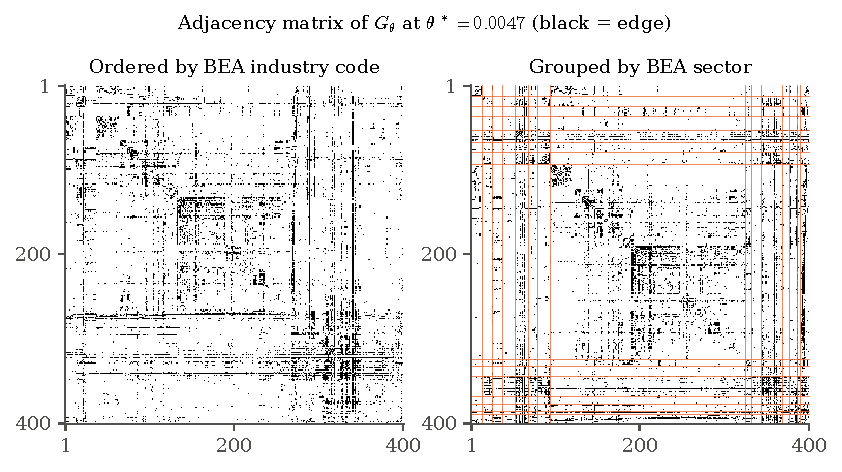
\includegraphics[width=0.9\linewidth]{figures/fig-adjacency.pdf}
\caption{The adjacency matrix of $G_{\theta^\ast}$, $\theta^\ast=\ThetaStar$,
with industries in order of BEA code (left) and grouped by BEA sector
(right; lines mark sector boundaries). Black entries are $1$. The dense rows
and columns are the hub industries, which trade with most other
industries.}
\label{fig:adjacency}
\end{figure}

\paragraph{The graph at $\theta^\ast$.} $G_{\theta^\ast}$ has \EdgesStar{}
edges and mean degree \MeanDegStar, but its degrees are very unequal: their
standard deviation is \SdDegStar, against \ERSdDeg{} for a random graph of the
same density, and the largest is \MaxDegStar. The highest degrees belong to
industries that trade with most other industries: \HubOne{}
(\HubOneDeg), \HubTwo{} (\HubTwoDeg), \HubThree{} (\HubThreeDeg) and \HubFour{}
(\HubFourDeg). They appear as the dense rows and columns in
Figure~\ref{fig:adjacency}. The graph has \ComponentsStar{} components; the
\IsolatedStar{} isolated vertices are BEA's ``customs duties'' and ``private
households'' industries, which have no intermediate inputs. Its clique number
is \CliqueStar. Edges are only mildly concentrated inside the fifteen BEA
sectors: \FracWithinSector\% of edges lie inside a sector, against
\FracWithinSectorExp\% of all pairs of industries.

\paragraph{Common neighbours.} Figure~\ref{fig:common-neighbours} applies the
instrument of Section~\ref{subsec:delta} to $G_{\theta^\ast}$. In the random
graph, $\mathcal L$ and $\mathcal M$ have the same distribution, as
Proposition~\ref{prop:er} requires, with mean $(N-2)p^2=\ERCommon$. In the
industry network they separate: adjacent pairs have on average
$\bar\lambda=\LambdaFitStar$ common neighbours and non-adjacent pairs
$\bar\mu=\MuFitStar$, a gap of $\bar\lambda-\bar\mu=\GapStar$. The gap lies in
$[\ERGapLoStar,\ERGapHiStar]$ for random graphs of this density and in
$[\DPGapLoStar,\DPGapHiStar]$ for graphs with the network's own degrees; for
$H(2,20)$ it is $\lambda-\mu=16$. So adjacency predicts shared trading
partners far better than in a random graph, and somewhat better than the
unequal degrees alone would produce, but less sharply than in the strongly
regular benchmark. Figure~\ref{fig:delta-sweep}(b) shows that the order holds
at every threshold: the gap exceeds both random ranges for every $\theta$ in
\RangeGapAboveDP.

\begin{figure}[htbp]
\centering
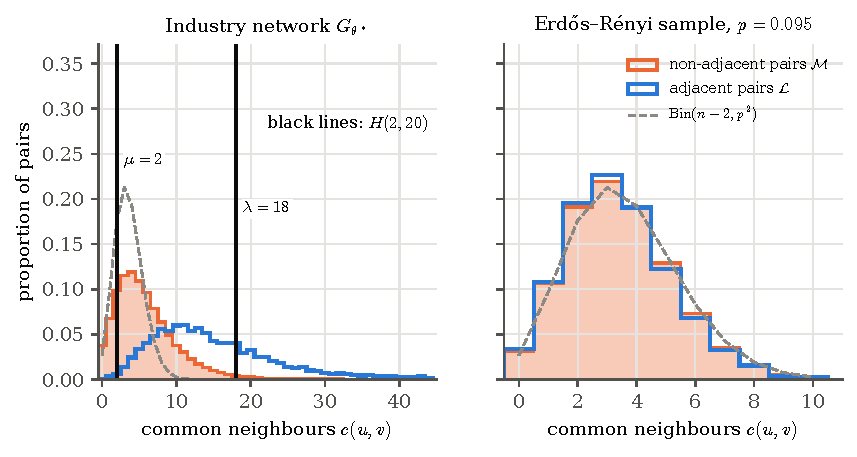
\includegraphics[width=0.95\linewidth]{figures/fig-common-neighbours.pdf}
\caption{Distributions of the common-neighbour counts $c(u,v)$ for adjacent
pairs ($\mathcal L$, blue) and non-adjacent pairs ($\mathcal M$, orange), in
$G_{\theta^\ast}$ (left) and in one Erd\H{o}s--R\'enyi graph of the same
density (right), with the distribution $\Bin(N-2,p^2)$ that
Proposition~\ref{prop:er} predicts for both lists in the random graph
(dashed). Black lines: the constant values $\lambda=18$ and $\mu=2$ of
$H(2,20)$.}
\label{fig:common-neighbours}
\end{figure}

\paragraph{Distance from strong regularity.} At $\theta^\ast$,
$\delta(G_{\theta^\ast})=\DeltaStar$. By Proposition~\ref{prop:residual} the
squared residual splits into three parts: \FracEdgeStar\% from the spread of
$\mathcal L$ (standard deviation \SdLambdaStar), \FracNonedgeStar\% from the
spread of $\mathcal M$ (standard deviation \SdMuStar), and only
\FracDegreeStar\% from the unequal degrees, large as they are. Random graphs of
the same density give $\delta$ in $[\ERDeltaLoStar,\ERDeltaHiStar]$, and
graphs with the same degrees give $[\DPDeltaLoStar,\DPDeltaHiStar]$. The
industry network is therefore further from strong regularity than a random
graph of its density, but slightly closer than a random graph with its
degrees. Figure~\ref{fig:delta-sweep}(a) shows the same order across the
sweep: $\delta(G_\theta)$ lies above the random-graph range for every $\theta$
in \RangeDeltaAboveER{} and below the degree-preserving range for every
$\theta$ in \RangeDeltaBelowDP.

\begin{figure}[htbp]
\centering
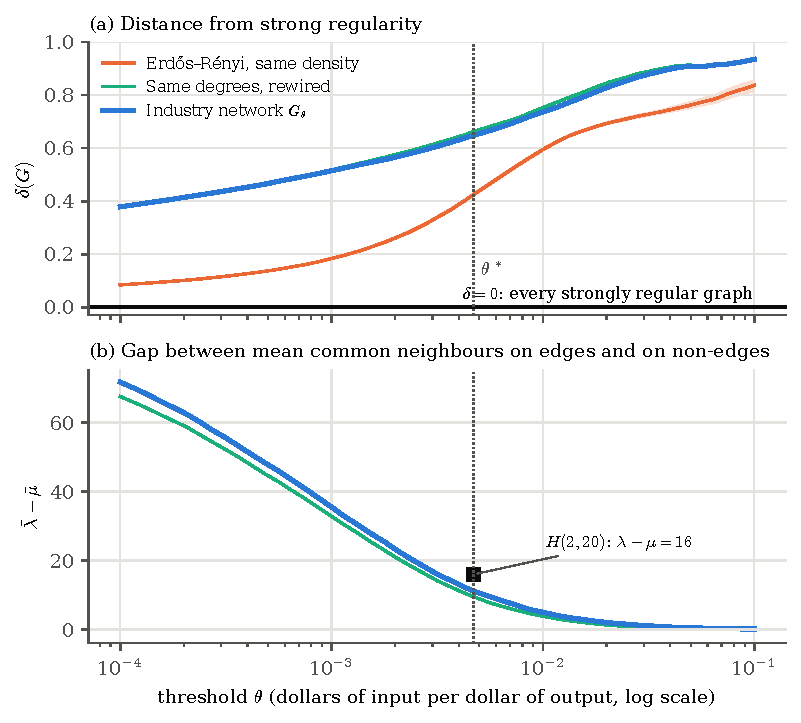
\includegraphics[width=0.9\linewidth]{figures/fig-delta-sweep.pdf}
\caption{(a) Distance from strong regularity $\delta(G_\theta)$ as the
threshold varies, for the industry network (blue), random graphs of the same
density (orange) and random graphs with the same degree sequence (green);
shading is the central $95\%$ range of the benchmarks. The line $\delta=0$ is
every strongly regular graph. (b) The gap $\bar\lambda-\bar\mu$ for the same
graphs, and $\lambda-\mu=16$ for $H(2,20)$. The dotted line marks
$\theta^\ast$. The horizontal axis is logarithmic.}
\label{fig:delta-sweep}
\end{figure}

\paragraph{Spectra.} Figure~\ref{fig:spectra} compares the adjacency spectra
at $\theta^\ast$. $H(2,20)$ has three distinct eigenvalues; the industry
network has \DistinctStar{} (to within $10^{-6}$) and the random graph
\ERDistinct, so on this count the industry network is as far from strong
regularity as a random graph. Its largest eigenvalue is \LambdaOneAStar,
against \ERLambdaOne{} for the random graph: a largest eigenvalue well above
the mean degree $38$ is what very unequal degrees produce, since it lies
between the mean and the maximum degree (Section~\ref{sec:spectra}).

\begin{figure}[htbp]
\centering
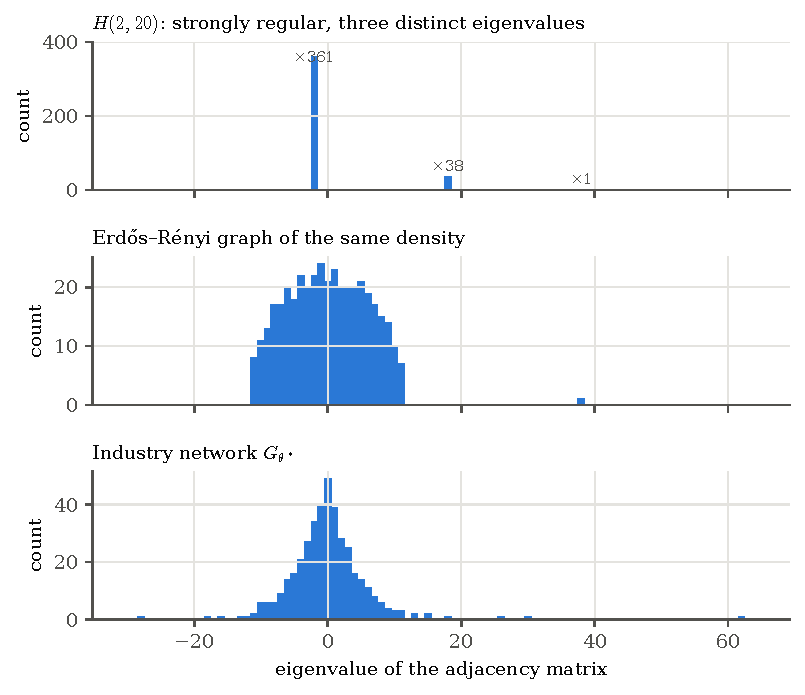
\includegraphics[width=0.85\linewidth]{figures/fig-spectra.pdf}
\caption{Adjacency spectra of $H(2,20)$ (three distinct eigenvalues, with
multiplicities), of one Erd\H{o}s--R\'enyi graph of the same density as
$G_{\theta^\ast}$, and of $G_{\theta^\ast}$.}
\label{fig:spectra}
\end{figure}

\begin{table}[htbp]
\centering
\small
\caption{The three graphs at $\theta^\ast=\ThetaStar$. The $H(2,20)$ column is
exact and $G_{\theta^\ast}$ is a computation on the 2017 tables. In the
Erd\H{o}s--R\'enyi column: (a) expected value, by construction; (b) one
sample; (c) the expectation $(N-2)p^2$ from Proposition~\ref{prop:er};
(d) mean over \NER{} samples.}
\label{tab:supply-summary}
\begin{tabular}{@{}lccc@{}}
\toprule
 & $H(2,20)$ & Erd\H{o}s--R\'enyi & $G_{\theta^\ast}$ \\
\midrule
Mean degree $\bar d$                 & $38$  & $38^{a}$             & $\MeanDegStar$ \\
Standard deviation of degree         & $0$   & $\ERSdDeg^{b}$       & $\SdDegStar$ \\
$\bar\lambda$                        & $18$  & $\ERCommon^{c}$      & $\LambdaFitStar$ \\
$\bar\mu$                            & $2$   & $\ERCommon^{c}$      & $\MuFitStar$ \\
$\bar\lambda-\bar\mu$                & $16$  & $\ERGapStar^{d}$     & $\GapStar$ \\
$\delta$                             & $0$   & $\ERDeltaStar^{d}$   & $\DeltaStar$ \\
Distinct eigenvalues of $A$          & $3$   & $\ERDistinct^{b}$    & $\DistinctStar$ \\
Largest eigenvalue of $A$            & $38$  & $\ERLambdaOne^{b}$   & $\LambdaOneAStar$ \\
Clique number                        & $20$  & $\ERClique^{b}$      & $\CliqueStar$ \\
\bottomrule
\end{tabular}
\end{table}

\paragraph{Stability over time.} The same analysis on the 2012 tables, at the
same level of detail, gives $\theta^\ast=\ThetaStarTwelve$, a gap
$\bar\lambda-\bar\mu=\GapTwelve$ (degree-preserving upper end \DPGapHiTwelve)
and $\delta=\DeltaTwelve$ (random-graph upper end \ERDeltaHiTwelve,
degree-preserving lower end \DPDeltaLoTwelve), the same pattern as in 2017.
At the coarser level of \NSummary{} industries, available for every year from
\YearFirst{} to \YearLast, we repeat the analysis at the threshold that matches
the density of $H(2,20)$ (Figure~\ref{fig:years}). In all \NYears{} years the
gap exceeds the degree-preserving range and $\delta$ lies between the two
random ranges. Across the years $\rho(A)$ stays between \YearsRhoMin{}
(\YearsRhoMinYear) and \YearsRhoMax{} (\YearsRhoMaxYear), and the average
supply-chain length between \YearsAPLMin{} and \YearsAPLMax{} steps.

\begin{figure}[htbp]
\centering
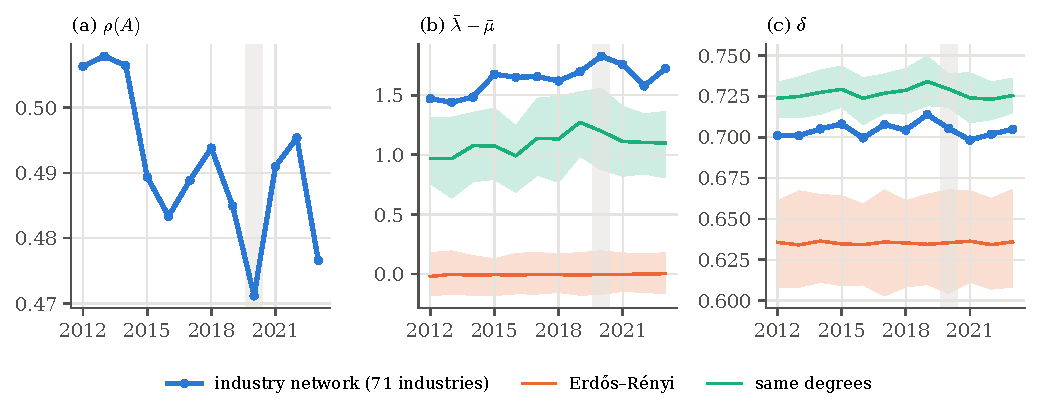
\includegraphics[width=\linewidth]{figures/fig-years.pdf}
\caption{Year by year, \YearFirst--\YearLast, for the \NSummary{}-industry
tables: (a) the spectral radius $\rho(A)$; (b) the gap $\bar\lambda-\bar\mu$
and (c) $\delta$, at the threshold matching the density of $H(2,20)$, with the
central $95\%$ ranges of the two random benchmarks. The year 2020 is shaded.}
\label{fig:years}
\end{figure}

\paragraph{Summary.} On these tables, supply chains are short: half of all
requirements are direct purchases, and the average chain is about two steps
long, with longer chains decaying at the rate $\rho(A)$. As a graph, the
network is dominated by a few service industries that supply most other
industries.
Even so, whether two industries trade directly predicts how many trading
partners they share more strongly than the unequal degrees alone would
produce. What separates the network from strong regularity is variation: the
number of shared partners varies greatly from one pair to the next, which
accounts for most of $\delta$. These are statements about the US input--output
tables over 2012--2023, not general facts about supply chains.

% ---------------------------------------------------------------------
\subsection{Limitations}
\label{subsec:supply-limits}

An industry aggregates many firms, so an edge between two industries does not
mean that any particular firms trade; firm-level supplier networks are not
publicly available. The tables record total requirements, including inputs
that were imported, so $A$ describes the technology of US production rather
than purely domestic supply chains. Thresholding discards both the size of
each requirement and its direction; we report a sweep of thresholds for the
first reason, and the directed matrix $A$ itself is used in
Section~\ref{subsec:walks}. Restricting to the $400$ largest industries treats
the two smallest as outside suppliers; no industry buys more than
\DroppedShare{} cents of inputs from them per dollar of its output. Finally, the benchmarks are deliberately extreme: a
network that sits between them is neither perfectly uniform nor random, which
is informative but is not a model of how supply chains form.
      % where the section goes
%  Requires amsmath, amssymb, amsthm, graphicx, booktabs, and the theorem
%  environments definition, theorem, proposition, corollary, remark, example.
%
%  Every number below is a macro from generated/numbers.tex, written by
%  scripts/run_analysis.py. Do not type numbers into this file by hand:
%  rerun the pipeline instead, and the text stays consistent with the code.
% =====================================================================

\providecommand{\R}{\mathbb{R}}
\providecommand{\tr}{\operatorname{tr}}
\providecommand{\Var}{\operatorname{Var}}
\providecommand{\Bin}{\operatorname{Bin}}
\providecommand{\fro}[1]{\lVert #1\rVert_F}
\providecommand{\1}{\mathbf{1}}

\section{An application: supply chains in the US economy}
\label{sec:supply}

Every industry buys inputs from other industries, which buy inputs from others
in turn. The resulting network of supply chains is recorded, for the whole US
economy, in the input--output accounts of the Bureau of Economic Analysis, and
it is the standard object for studying how a disruption in one industry
travels to others \cite{acemoglu2012,carvalho2014}. This
section applies the article's machinery to that network in two ways. First, the
theorem that powers of an adjacency matrix count walks (Theorem~\ref{thm:walks})
has a weighted form, and in that form it \emph{is} the standard description of
how requirements travel along supply chains. Second, the definition of strong
regularity becomes a measuring instrument: we build a graph from the network and
measure how far it is from strongly regular, using random graphs and a strongly
regular graph as benchmarks. Strongly regular graphs do not occur in economic
data, and nothing here claims that they do.

Table~\ref{tab:supply-status} records how strong each connection is, so that a
reader can tell a theorem from a modelling choice.

\begin{table}[htbp]
\centering
\small
\caption{Strength of each link between the article's mathematics and the
supply-chain application.}
\label{tab:supply-status}
\begin{tabular}{@{}p{0.44\linewidth}p{0.17\linewidth}p{0.31\linewidth}@{}}
\toprule
Connection & Status & Support \\
\midrule
Powers of $A$ count weighted supply chains & Direct & Theorem~\ref{thm:weighted-walks} (proved here) \\
Total requirements $=\sum_k A^k$ & Direct & Theorem~\ref{thm:neumann} (proved here) \\
Average supply-chain length & Direct & Proposition~\ref{prop:chain-length} (proved here) \\
$(A_\theta^2)_{uv}$ counts common neighbours & Direct & Theorem~\ref{thm:walks} \\
Distance from strong regularity, $\delta(G)$ & Direct & Proposition~\ref{prop:residual} (proved here) \\
Erd\H{o}s--R\'enyi graph as a null model & Benchmark & Proposition~\ref{prop:er} (proved here) \\
Graphs with the same degree sequence & Benchmark & Computation \\
Strongly regular graph $H(2,20)$ & Benchmark & Corollary~\ref{cor:delta-zero} \\
Industries as stand-ins for firms & Approximation & Industries aggregate many firms \\
\bottomrule
\end{tabular}
\end{table}

% ---------------------------------------------------------------------
\subsection{The data: requirements between industries}
\label{subsec:io-data}

The Bureau of Economic Analysis records, for each year, how much of each
commodity every industry buys (the \emph{Use} table) and how much of each
commodity every industry produces (the \emph{Make} table), in millions of
dollars \cite{horowitz2009}. We use the tables at producer prices, before
redefinitions, in the 2017 industry classification, as redistributed
in the U.S. Environmental Protection Agency's open-source package
\texttt{useeior} \cite{li2022useeior,bea2025io}. From them we form the
standard industry-by-industry matrix \cite[Ch.~5]{miller2009}.

\begin{definition}[Direct requirements]
\label{def:direct}
Let $U$ be the commodity-by-industry matrix of intermediate purchases, $V$ the
industry-by-commodity matrix of production, $g=V\1$ the vector of industry
outputs and $q=V^{\mathsf T}\1$ the vector of commodity outputs. Every
industry has $g_j>0$; let $B=U\,\mathrm{diag}(g)^{-1}$, and let $D$ have
entries $d_{ic}=v_{ic}/q_c$, with $d_{ic}=0$ when $q_c=0$ (a few commodities,
such as used goods, are produced by no industry). The
\emph{direct-requirements matrix} is $A=DB$. Its entry $a_{ij}\ge 0$ is the
number of dollars of industry $i$'s output used directly to produce one dollar
of industry $j$'s output.
\end{definition}

Column $j$ of $A$ is industry $j$'s recipe of intermediate inputs per dollar
of output; the rest of each dollar pays for labour, capital, taxes and imports
not produced by any US industry. We take the $N=\NInd$ industries with the
largest gross output in 2017, out of \NIndSource, numbered $1,\dots,N$ in
order of their BEA industry code; this ordering is used for every matrix in
this section. We work mainly with 2017, and repeat the analysis for 2012 at
this level and for every year from \YearFirst{} to \YearLast{} at the coarser
level of \NSummary{} industries. In each Use table a handful of entries are
negative (in the 2017 detail table, for example, entries for used and
secondhand goods and for a few farm and food products); we set them to zero,
so that $A$ is entrywise non-negative. All
computations in this section are on these public tables and are labelled as
such. The code that produces every number, table and figure is publicly
available.\footnote{\url{https://github.com/desaidaksh1206-netizen/supply-chain-graphs-srg}}

% ---------------------------------------------------------------------
\subsection{Supply chains are weighted walks}
\label{subsec:walks}

Regard $A$ as a weighted adjacency matrix of a directed graph on the
industries, with an arc $i\to j$ of weight $a_{ij}$ whenever $a_{ij}>0$: an arc
points from a supplier to a buyer. A \emph{supply chain of length $k$} from $i$
to $j$ is a walk $i=v_0\to v_1\to\dots\to v_k=j$, and its \emph{weight} is the
product $a_{v_0v_1}a_{v_1v_2}\cdots a_{v_{k-1}v_k}$.

\begin{theorem}[Weighted walks]
\label{thm:weighted-walks}
For every $k\ge1$, $(A^k)_{ij}$ is the sum of the weights of all walks of
length $k$ from $i$ to $j$.
\end{theorem}

\begin{proof}
For $k=1$ the only walk of length one from $i$ to $j$ is the arc itself, of
weight $a_{ij}$. Suppose the statement holds for $k$. Every walk of length
$k+1$ from $i$ to $j$ is a walk of length $k$ from $i$ to some vertex $\ell$,
followed by the arc $\ell\to j$, and its weight is the product of the two
weights. Summing over $\ell$ and using the induction hypothesis,
$\sum_\ell (A^k)_{i\ell}\,a_{\ell j}=(A^{k+1})_{ij}$.
\end{proof}

With all weights equal to $1$ this is Theorem~\ref{thm:walks}. The weighted
form has a direct reading: to make one dollar of $j$'s output, industry $j$
uses $a_{\ell j}$ dollars from each supplier $\ell$, each of which uses
$a_{i\ell}$ dollars of $i$'s output per dollar, and so on back along the chain.
So $(A^k)_{ij}$ is the amount of $i$'s output, in dollars, that one dollar of
$j$'s output requires through chains with exactly $k-1$ intermediate
industries.

\begin{theorem}[Total requirements]
\label{thm:neumann}
Let $A\ge0$ have spectral radius $\rho(A)<1$. Then $I-A$ is invertible,
\begin{equation}\label{eq:neumann}
  L=(I-A)^{-1}=I+A+A^2+A^3+\cdots,
\end{equation}
and every entry of $L$ is non-negative.
\end{theorem}

\begin{proof}
Because $\rho(A)<1$, $A^k\to0$ as $k\to\infty$ \cite[Sec.~5.6]{horn2013}.
For each $k$,
$(I-A)(I+A+\dots+A^k)=I-A^{k+1}$. If $(I-A)x=0$ then $x=A^{k+1}x\to0$, so
$x=0$ and $I-A$ is invertible. Multiplying by $(I-A)^{-1}$ gives
$I+A+\dots+A^k=(I-A)^{-1}(I-A^{k+1})\to(I-A)^{-1}$. Every partial sum is
non-negative, so the limit is.
\end{proof}

$L$ is the Leontief inverse \cite{leontief1936}. By
Theorem~\ref{thm:weighted-walks}, $L_{ij}$ adds up the requirements of one
dollar of $j$'s output for $i$'s output along supply chains of every length.
Its column sums are the \emph{output multipliers}: the total output, across
the economy, needed to deliver one dollar of $j$'s product to final users
\cite[Ch.~6]{miller2009}.

The hypothesis $\rho(A)<1$ is often checked through the following bound.

\begin{proposition}\label{prop:colsum}
For any real square matrix, $\rho(A)\le\max_j\sum_i|a_{ij}|$.
\end{proposition}

\begin{proof}
Let $Av=\lambda v$ with $v\ne0$, and write $\|x\|_1=\sum_i|x_i|$. Then
\[
  |\lambda|\,\|v\|_1=\|Av\|_1\le\sum_j|v_j|\sum_i|a_{ij}|
  \le\Bigl(\max_j\sum_i|a_{ij}|\Bigr)\|v\|_1 ,
\]
and dividing by $\|v\|_1>0$ gives the bound for every eigenvalue.
\end{proof}

Since column $j$ of $A$ sums to the share of $j$'s output spent on
intermediate inputs, one expects every column sum to be below $1$. On our data
that fails for exactly \NColAboveOne{} industry, state and local government
passenger transit: its value added is negative in the tables, and its
intermediate purchases are \MaxColSum{} times the value of its output.
Proposition~\ref{prop:colsum} therefore does not apply. We compute $\rho(A)$ directly instead:
$\rho(A)=\Rho$ for 2017 and \RhoTwelve{} for 2012, so
Theorem~\ref{thm:neumann} holds. The partial sum $I+A+\dots+A^{20}$ of
\eqref{eq:neumann} is within $\NeumannTwenty$ of $L$, entry by entry.

\begin{proposition}[Average supply-chain length]
\label{prop:chain-length}
Let $A\ge0$ with $\rho(A)<1$ and $A\ne0$, and let
$s_k=\1^{\mathsf T}A^k\1\big/\1^{\mathsf T}(L-I)\1$ for $k\ge1$. Then
$\sum_{k\ge1}s_k=1$ and
\[
  \sum_{k\ge1}k\,s_k=\frac{\1^{\mathsf T}(L-I)L\,\1}{\1^{\mathsf T}(L-I)\1}.
\]
\end{proposition}

\begin{proof}
By \eqref{eq:neumann}, $L-I=\sum_{k\ge1}A^k$, which gives the first claim.
By Gelfand's formula $\rho(A)=\lim_{k\to\infty}\lVert A^k\rVert^{1/k}$
\cite[Sec.~5.6]{horn2013}, for any $r$ with $\rho(A)<r<1$ there is a constant
$C$ with $\lVert A^k\rVert\le Cr^k$ for all $k$, so $\sum_{k\ge1}kA^{k}$
converges absolutely. Its terms are non-negative, so it can be rearranged:
$\sum_{k\ge1}kA^k=\sum_{k\ge1}\sum_{j\ge k}A^j=\sum_{k\ge1}A^k L=(L-I)L$,
since $\sum_{j\ge k}A^j=A^kL$.
\end{proof}

So $s_k$ is the share of all requirements, direct and indirect, that travels
along chains of exactly $k$ steps, and $\sum_k k s_k$ is the average length of
a supply chain weighted by the dollars it carries; it is an economy-wide
version of the average propagation length of \cite{dietzenbacher2005}.

Figure~\ref{fig:walks} shows the result (computation). Direct purchases carry
$s_1=\ShareOne\%$ of all requirements, two-step chains $\ShareTwo\%$, three-step
chains $\ShareThree\%$, and chains of four or more steps the remaining
$\ShareBeyondThree\%$. The average supply-chain length is \APL{} steps
(\APLTwelve{} in 2012). Successive shares shrink by a nearly constant factor:
$s_{k+1}/s_k$ lies between \RatioMin{} and \RatioMax{} for $k=1,\dots,8$,
close to $\rho(A)=\Rho$. This is what one expects: by Perron--Frobenius
theory, $\rho(A)$ is itself an eigenvalue of the non-negative matrix $A$, with
a non-negative eigenvector \cite[Sec.~8.3]{horn2013}, and the largest
eigenvalue sets the rate at which $A^k$ decays. Output
multipliers range from \MultMin{} to \MultMax, with mean \MultMean: on average,
delivering a dollar of final product requires about two dollars of output across
the economy.

\begin{figure}[htbp]
\centering
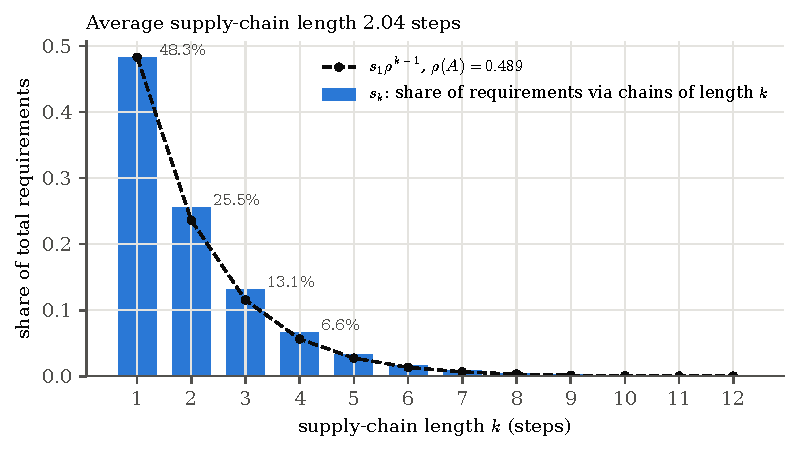
\includegraphics[width=0.85\linewidth]{figures/fig-walks.pdf}
\caption{Share $s_k$ of all requirements carried by supply chains of exactly
$k$ steps (bars), with the geometric decay $s_1\rho(A)^{k-1}$ (dashed), for
the \NInd{} industries in 2017. Computation on the BEA tables of
Section~\ref{subsec:io-data}.}
\label{fig:walks}
\end{figure}

% ---------------------------------------------------------------------
\subsection{From requirements to a graph}
\label{subsec:threshold}

To ask how \emph{structured} the network is, we turn $A$ into a simple graph
of the kind studied in this article.

\begin{definition}[Threshold graph]
\label{def:threshold}
Let $w_{ij}=\max(a_{ij},a_{ji})$ for $i\ne j$. For $\theta>0$, the
\emph{threshold graph} $G_\theta$ has vertex set $\{1,\dots,N\}$, with $i\ne j$
adjacent if and only if $w_{ij}\ge\theta$, that is, if one of the two
industries buys at least $\theta$ dollars from the other per dollar of its own
output. Its adjacency matrix is $A_\theta$.
\end{definition}

Lowering $\theta$ adds edges and never removes them. No threshold is
privileged, so the two measures defined in Section~\ref{subsec:delta}, $\delta$
and $\bar\lambda-\bar\mu$, are reported over \NThetas{} thresholds spaced evenly
on a logarithmic scale from $10^{-4}$ (a hundredth of a cent per dollar) to
$10^{-1}$ (ten cents per dollar). The other quantities are reported at the
threshold at which $G_\theta$ has the density of $H(2,20)$, defined in
Section~\ref{subsec:benchmarks}.

% ---------------------------------------------------------------------
\subsection{Measuring distance from strong regularity}
\label{subsec:delta}

Let $G$ be a graph on $n$ vertices with adjacency matrix $A$, and write
$\bar A=J-I-A$ for the adjacency matrix of its complement. (In this subsection
and the next, $A$ is a $0/1$ adjacency matrix.) By Theorem~\ref{thm:walks},
for $u\ne v$ the entry $(A^2)_{uv}$ is the number of common neighbours of $u$
and $v$; we write $c(u,v)=(A^2)_{uv}$. The diagonal entry $(A^2)_{uu}$ is the
degree $d(u)$. Recall from Section~\ref{sec:srg} that $G$, neither complete nor
edgeless, is strongly regular with parameters $(n,k,\lambda,\mu)$ exactly when
\begin{equation}\label{eq:srg-identity}
  A^2=kI+\lambda A+\mu\bar A .
\end{equation}
The three matrices $I$, $A$, $\bar A$ have disjoint supports: $I$ covers the
diagonal, $A$ the ordered adjacent pairs, $\bar A$ the ordered non-adjacent
pairs. Equation \eqref{eq:srg-identity} therefore says three things at once:
every diagonal entry of $A^2$ equals $k$, every entry on an edge equals
$\lambda$, and every entry on a non-edge equals $\mu$. For a general graph
these entries are not constant. They form three lists:
\begin{equation}\label{eq:three-lists}
  \mathcal D=\bigl(d(u)\bigr)_{u},\qquad
  \mathcal L=\bigl(c(u,v)\bigr)_{u\sim v},\qquad
  \mathcal M=\bigl(c(u,v)\bigr)_{u\not\sim v,\,u\ne v},
\end{equation}
indexed by vertices, ordered adjacent pairs, and ordered distinct non-adjacent
pairs respectively. If $G$ has $m$ edges and $\bar m$ non-edges, the lists have
lengths $n$, $2m$ and $2\bar m$. Write $\bar d,\bar\lambda,\bar\mu$ for their
means and $\Var$ for the population variance of a list.

\begin{proposition}\label{prop:residual}
Let $G$ have at least one edge and at least one non-edge. For real
$k,\lambda,\mu$ let $R(k,\lambda,\mu)=A^2-kI-\lambda A-\mu\bar A$. Then
\begin{equation}\label{eq:residual}
  \min_{k,\lambda,\mu\in\R}\fro{R(k,\lambda,\mu)}^2
  = n\Var(\mathcal D)+2m\Var(\mathcal L)+2\bar m\Var(\mathcal M),
\end{equation}
and the minimum is attained exactly at $(k,\lambda,\mu)=(\bar d,\bar\lambda,\bar\mu)$.
\end{proposition}

\begin{proof}
Because $I$, $A$ and $\bar A$ have disjoint supports that together cover every
entry, the squared Frobenius norm splits as
\[
  \fro{R}^2=\sum_{u}\bigl(d(u)-k\bigr)^2
  +\sum_{u\sim v}\bigl(c(u,v)-\lambda\bigr)^2
  +\sum_{u\not\sim v,\,u\ne v}\bigl(c(u,v)-\mu\bigr)^2 ,
\]
with the last two sums over ordered pairs. Each term involves only one of
$k,\lambda,\mu$, so each can be minimised separately. For a list
$x_1,\dots,x_\ell$ and real $a$,
$\sum_i(x_i-a)^2=\ell\Var(x)+\ell(\bar x-a)^2$, which is minimised exactly at
$a=\bar x$ with minimum $\ell\Var(x)$. Applying this to each list gives
\eqref{eq:residual}.
\end{proof}

\begin{definition}[Distance from strong regularity]
\label{def:delta}
For $G$ with at least one edge and one non-edge, set
\[
  \delta(G)=\frac{\min_{k,\lambda,\mu}\fro{R(k,\lambda,\mu)}}{\fro{A^2}} .
\]
\end{definition}

Taking $k=\lambda=\mu=0$ gives $R=A^2$, so $0\le\delta(G)\le1$. The
normalisation makes $\delta$ comparable across thresholds, where the number of
edges changes.

\begin{corollary}\label{cor:delta-zero}
Let $G$ be neither complete nor edgeless. Then $\delta(G)=0$ if and only if
$G$ is strongly regular, in which case $(\bar d,\bar\lambda,\bar\mu)$ are its
parameters $(k,\lambda,\mu)$.
\end{corollary}

\begin{proof}
By Proposition~\ref{prop:residual}, $\delta(G)=0$ if and only if all three
lists in \eqref{eq:three-lists} are constant, which is \eqref{eq:srg-identity}
with $(k,\lambda,\mu)=(\bar d,\bar\lambda,\bar\mu)$.
\end{proof}

The degree term in \eqref{eq:residual} cannot be dropped: constant $\lambda$
and constant $\mu$ do not by themselves force a graph to be regular.

\begin{example}[The bow-tie]
\label{ex:bowtie}
Let $G$ be two triangles sharing one vertex, with vertices ordered
$v_0,v_1,v_2,v_3,v_4$, where $v_0$ is the shared vertex and the triangles are
$\{v_0,v_1,v_2\}$ and $\{v_0,v_3,v_4\}$. Then
\[
  A=\begin{pmatrix}
  0&1&1&1&1\\ 1&0&1&0&0\\ 1&1&0&0&0\\ 1&0&0&0&1\\ 1&0&0&1&0
  \end{pmatrix},
  \qquad
  A^2=\begin{pmatrix}
  4&1&1&1&1\\ 1&2&1&1&1\\ 1&1&2&1&1\\ 1&1&1&2&1\\ 1&1&1&1&2
  \end{pmatrix}.
\]
Every off-diagonal entry of $A^2$ is $1$, so $\mathcal L$ and $\mathcal M$ are
constant with $\lambda=\mu=1$. The degrees are $4,2,2,2,2$, so
$\bar d=12/5$, $\Var(\mathcal D)=32/5-(12/5)^2=16/25$, and by
\eqref{eq:residual} the minimum squared residual is $5\cdot16/25=16/5$.
The graph is not strongly regular, and only the degree term detects it.
By the friendship theorem of Erd\H{o}s, R\'enyi and S\'os
\cite{erdos1966friendship}, the finite graphs in which every two distinct
vertices have exactly one common neighbour are precisely the graphs consisting
of triangles sharing a common vertex, so the bow-tie is the smallest graph
with $\lambda=\mu=1$ that is not regular. Other values give smaller examples:
the path $v_1v_2v_3$ has $\lambda=0$ and $\mu=1$, with degrees $1,2,1$.
\end{example}

% ---------------------------------------------------------------------
\subsection{The benchmarks}
\label{subsec:benchmarks}

\paragraph{Random graphs.} The random graph $G(n,p)$ of Gilbert
\cite{gilbert1959}, usually called the Erd\H{o}s--R\'enyi model, includes each
of the $\binom n2$ possible edges independently with probability $p$. Erd\H{o}s
and R\'enyi \cite{erdos1959} studied the closely related model with a fixed
number of edges.

\begin{proposition}\label{prop:er}
In $G(n,p)$, each degree $d(u)$ has distribution $\Bin(n-1,p)$. For distinct
$u,v$, the count $c(u,v)$ has distribution $\Bin(n-2,p^2)$ and is independent
of whether $u$ and $v$ are adjacent.
\end{proposition}

\begin{proof}
The degree of $u$ counts which of the $n-1$ independent edges at $u$ are
present. For $u\ne v$, a third vertex $w$ is a common neighbour exactly when
both $uw$ and $vw$ are edges, which has probability $p^2$; these events for the
$n-2$ choices of $w$ involve disjoint pairs of edges and so are independent.
None of them involves the edge $uv$, so $c(u,v)$ is independent of it.
\end{proof}

So in a random graph, adjacency tells us nothing about common neighbours:
$\mathcal L$ and $\mathcal M$ have the same distribution, and
$\bar\lambda-\bar\mu$ is close to zero.

\paragraph{Graphs with the same degrees.} A random graph differs from
$G_\theta$ in two ways at once: its degrees are nearly equal, and its edges
are placed independently. To separate the two, we also compare with random
graphs that have \emph{exactly} the degree sequence of $G_\theta$, generated by
repeated double-edge swaps \cite{maslov2002}: two edges $\{a,b\}$ and $\{c,d\}$
are replaced by $\{a,d\}$ and $\{c,b\}$ whenever this creates no loop or
repeated edge, which leaves every degree unchanged. We make five swap attempts
per edge. This benchmark is a computation; we prove nothing about it.

For each $\theta$ we report the mean and the central $95\%$ range of $\delta$
and of $\bar\lambda-\bar\mu$ over \NER{} Erd\H{o}s--R\'enyi graphs with the
density of $G_\theta$, and over \NDP{} degree-preserving rewirings of
$G_\theta$ (\NDPStar{} at $\theta^\ast$ below). These ranges are computations,
not theorems.

\paragraph{A strongly regular graph.} By Corollary~\ref{cor:delta-zero}, every
strongly regular graph has $\delta=0$. For the spectral comparison we want a
specific strongly regular graph of the same order. Choosing $N=400$ makes one
available from Section~\ref{sec:johnson-hamming}: the Hamming graph $H(2,20)$
\cite[Example~2.2.2]{mentorthesis}, whose vertices are the pairs $(a,b)$ with
$a,b\in\{0,\dots,19\}$, adjacent when they differ in exactly one coordinate.
Its parameters are
$(n,k,\lambda,\mu)=(400,38,18,2)$, its non-trivial eigenvalues are the roots of
$x^2-(\lambda-\mu)x+(\mu-k)=x^2-16x-36$ \cite{brouwer2012}, namely $18$ and $-2$, with
multiplicities $38$ and $361$ (one checks $38+38\cdot18-361\cdot2=0=\tr A$),
and its largest cliques are its $40$ ``lines'' of $20$ vertices. We write
$\theta^\ast$ for the threshold at which $G_\theta$ has exactly the density of
$H(2,20)$, hence mean degree $38$; on our data
$\theta^\ast=\ThetaStar$, that is, \ThetaStarCents{} cents per dollar.

% ---------------------------------------------------------------------
\subsection{Results}
\label{subsec:supply-results}

All numbers and figures in this subsection are computations on the 2017 BEA
tables, except where another year is named. Figure~\ref{fig:adjacency} shows
the adjacency matrix of $G_{\theta^\ast}$, first in the ordering by industry
code used throughout and then with the industries grouped by sector. The two
matrices are $A_{\theta^\ast}$ and $PA_{\theta^\ast}P^{\mathsf T}$ for a
permutation matrix $P$, so they describe the same graph.

\begin{figure}[htbp]
\centering
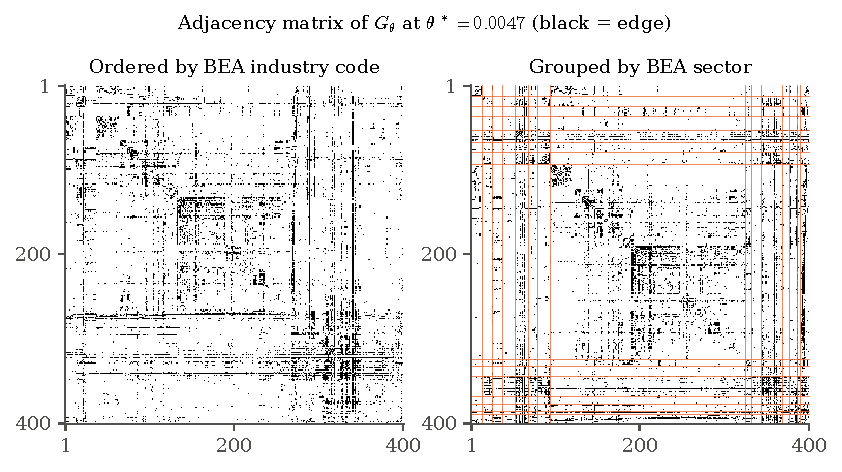
\includegraphics[width=0.9\linewidth]{figures/fig-adjacency.pdf}
\caption{The adjacency matrix of $G_{\theta^\ast}$, $\theta^\ast=\ThetaStar$,
with industries in order of BEA code (left) and grouped by BEA sector
(right; lines mark sector boundaries). Black entries are $1$. The dense rows
and columns are the hub industries, which trade with most other
industries.}
\label{fig:adjacency}
\end{figure}

\paragraph{The graph at $\theta^\ast$.} $G_{\theta^\ast}$ has \EdgesStar{}
edges and mean degree \MeanDegStar, but its degrees are very unequal: their
standard deviation is \SdDegStar, against \ERSdDeg{} for a random graph of the
same density, and the largest is \MaxDegStar. The highest degrees belong to
industries that trade with most other industries: \HubOne{}
(\HubOneDeg), \HubTwo{} (\HubTwoDeg), \HubThree{} (\HubThreeDeg) and \HubFour{}
(\HubFourDeg). They appear as the dense rows and columns in
Figure~\ref{fig:adjacency}. The graph has \ComponentsStar{} components; the
\IsolatedStar{} isolated vertices are BEA's ``customs duties'' and ``private
households'' industries, which have no intermediate inputs. Its clique number
is \CliqueStar. Edges are only mildly concentrated inside the fifteen BEA
sectors: \FracWithinSector\% of edges lie inside a sector, against
\FracWithinSectorExp\% of all pairs of industries.

\paragraph{Common neighbours.} Figure~\ref{fig:common-neighbours} applies the
instrument of Section~\ref{subsec:delta} to $G_{\theta^\ast}$. In the random
graph, $\mathcal L$ and $\mathcal M$ have the same distribution, as
Proposition~\ref{prop:er} requires, with mean $(N-2)p^2=\ERCommon$. In the
industry network they separate: adjacent pairs have on average
$\bar\lambda=\LambdaFitStar$ common neighbours and non-adjacent pairs
$\bar\mu=\MuFitStar$, a gap of $\bar\lambda-\bar\mu=\GapStar$. The gap lies in
$[\ERGapLoStar,\ERGapHiStar]$ for random graphs of this density and in
$[\DPGapLoStar,\DPGapHiStar]$ for graphs with the network's own degrees; for
$H(2,20)$ it is $\lambda-\mu=16$. So adjacency predicts shared trading
partners far better than in a random graph, and somewhat better than the
unequal degrees alone would produce, but less sharply than in the strongly
regular benchmark. Figure~\ref{fig:delta-sweep}(b) shows that the order holds
at every threshold: the gap exceeds both random ranges for every $\theta$ in
\RangeGapAboveDP.

\begin{figure}[htbp]
\centering
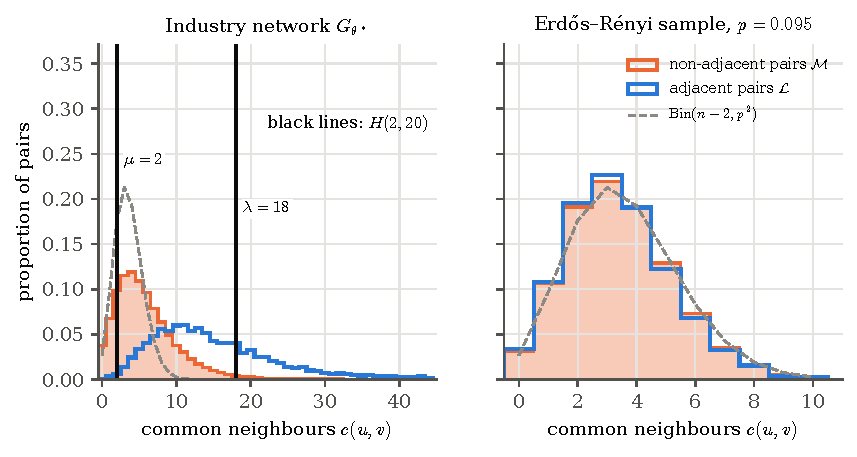
\includegraphics[width=0.95\linewidth]{figures/fig-common-neighbours.pdf}
\caption{Distributions of the common-neighbour counts $c(u,v)$ for adjacent
pairs ($\mathcal L$, blue) and non-adjacent pairs ($\mathcal M$, orange), in
$G_{\theta^\ast}$ (left) and in one Erd\H{o}s--R\'enyi graph of the same
density (right), with the distribution $\Bin(N-2,p^2)$ that
Proposition~\ref{prop:er} predicts for both lists in the random graph
(dashed). Black lines: the constant values $\lambda=18$ and $\mu=2$ of
$H(2,20)$.}
\label{fig:common-neighbours}
\end{figure}

\paragraph{Distance from strong regularity.} At $\theta^\ast$,
$\delta(G_{\theta^\ast})=\DeltaStar$. By Proposition~\ref{prop:residual} the
squared residual splits into three parts: \FracEdgeStar\% from the spread of
$\mathcal L$ (standard deviation \SdLambdaStar), \FracNonedgeStar\% from the
spread of $\mathcal M$ (standard deviation \SdMuStar), and only
\FracDegreeStar\% from the unequal degrees, large as they are. Random graphs of
the same density give $\delta$ in $[\ERDeltaLoStar,\ERDeltaHiStar]$, and
graphs with the same degrees give $[\DPDeltaLoStar,\DPDeltaHiStar]$. The
industry network is therefore further from strong regularity than a random
graph of its density, but slightly closer than a random graph with its
degrees. Figure~\ref{fig:delta-sweep}(a) shows the same order across the
sweep: $\delta(G_\theta)$ lies above the random-graph range for every $\theta$
in \RangeDeltaAboveER{} and below the degree-preserving range for every
$\theta$ in \RangeDeltaBelowDP.

\begin{figure}[htbp]
\centering
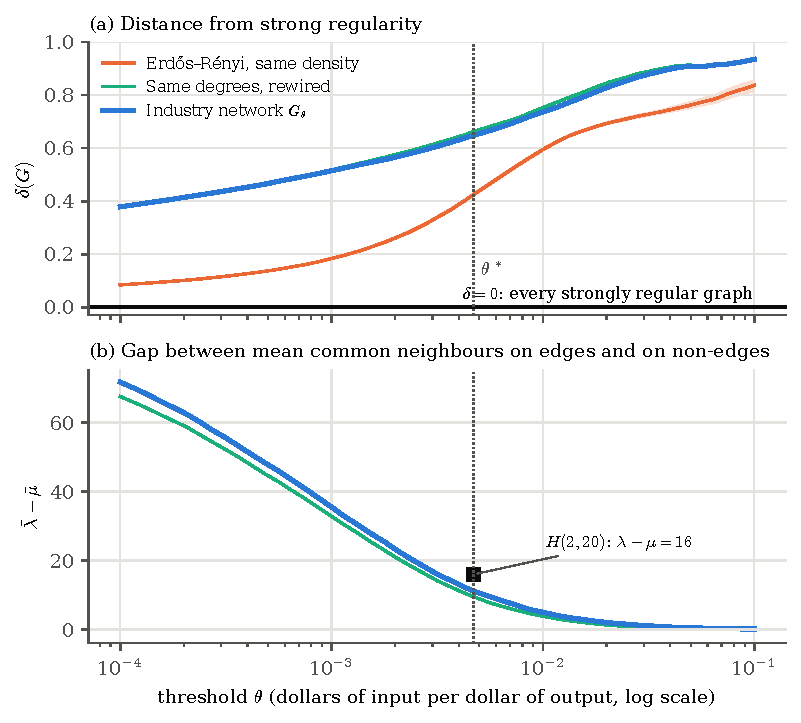
\includegraphics[width=0.9\linewidth]{figures/fig-delta-sweep.pdf}
\caption{(a) Distance from strong regularity $\delta(G_\theta)$ as the
threshold varies, for the industry network (blue), random graphs of the same
density (orange) and random graphs with the same degree sequence (green);
shading is the central $95\%$ range of the benchmarks. The line $\delta=0$ is
every strongly regular graph. (b) The gap $\bar\lambda-\bar\mu$ for the same
graphs, and $\lambda-\mu=16$ for $H(2,20)$. The dotted line marks
$\theta^\ast$. The horizontal axis is logarithmic.}
\label{fig:delta-sweep}
\end{figure}

\paragraph{Spectra.} Figure~\ref{fig:spectra} compares the adjacency spectra
at $\theta^\ast$. $H(2,20)$ has three distinct eigenvalues; the industry
network has \DistinctStar{} (to within $10^{-6}$) and the random graph
\ERDistinct, so on this count the industry network is as far from strong
regularity as a random graph. Its largest eigenvalue is \LambdaOneAStar,
against \ERLambdaOne{} for the random graph: a largest eigenvalue well above
the mean degree $38$ is what very unequal degrees produce, since it lies
between the mean and the maximum degree (Section~\ref{sec:spectra}).

\begin{figure}[htbp]
\centering
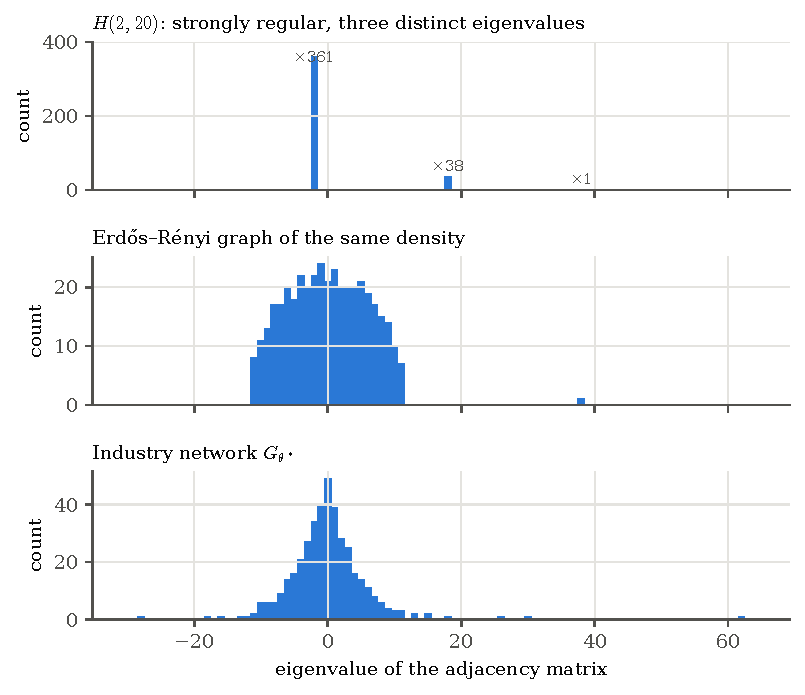
\includegraphics[width=0.85\linewidth]{figures/fig-spectra.pdf}
\caption{Adjacency spectra of $H(2,20)$ (three distinct eigenvalues, with
multiplicities), of one Erd\H{o}s--R\'enyi graph of the same density as
$G_{\theta^\ast}$, and of $G_{\theta^\ast}$.}
\label{fig:spectra}
\end{figure}

\begin{table}[htbp]
\centering
\small
\caption{The three graphs at $\theta^\ast=\ThetaStar$. The $H(2,20)$ column is
exact and $G_{\theta^\ast}$ is a computation on the 2017 tables. In the
Erd\H{o}s--R\'enyi column: (a) expected value, by construction; (b) one
sample; (c) the expectation $(N-2)p^2$ from Proposition~\ref{prop:er};
(d) mean over \NER{} samples.}
\label{tab:supply-summary}
\begin{tabular}{@{}lccc@{}}
\toprule
 & $H(2,20)$ & Erd\H{o}s--R\'enyi & $G_{\theta^\ast}$ \\
\midrule
Mean degree $\bar d$                 & $38$  & $38^{a}$             & $\MeanDegStar$ \\
Standard deviation of degree         & $0$   & $\ERSdDeg^{b}$       & $\SdDegStar$ \\
$\bar\lambda$                        & $18$  & $\ERCommon^{c}$      & $\LambdaFitStar$ \\
$\bar\mu$                            & $2$   & $\ERCommon^{c}$      & $\MuFitStar$ \\
$\bar\lambda-\bar\mu$                & $16$  & $\ERGapStar^{d}$     & $\GapStar$ \\
$\delta$                             & $0$   & $\ERDeltaStar^{d}$   & $\DeltaStar$ \\
Distinct eigenvalues of $A$          & $3$   & $\ERDistinct^{b}$    & $\DistinctStar$ \\
Largest eigenvalue of $A$            & $38$  & $\ERLambdaOne^{b}$   & $\LambdaOneAStar$ \\
Clique number                        & $20$  & $\ERClique^{b}$      & $\CliqueStar$ \\
\bottomrule
\end{tabular}
\end{table}

\paragraph{Stability over time.} The same analysis on the 2012 tables, at the
same level of detail, gives $\theta^\ast=\ThetaStarTwelve$, a gap
$\bar\lambda-\bar\mu=\GapTwelve$ (degree-preserving upper end \DPGapHiTwelve)
and $\delta=\DeltaTwelve$ (random-graph upper end \ERDeltaHiTwelve,
degree-preserving lower end \DPDeltaLoTwelve), the same pattern as in 2017.
At the coarser level of \NSummary{} industries, available for every year from
\YearFirst{} to \YearLast, we repeat the analysis at the threshold that matches
the density of $H(2,20)$ (Figure~\ref{fig:years}). In all \NYears{} years the
gap exceeds the degree-preserving range and $\delta$ lies between the two
random ranges. Across the years $\rho(A)$ stays between \YearsRhoMin{}
(\YearsRhoMinYear) and \YearsRhoMax{} (\YearsRhoMaxYear), and the average
supply-chain length between \YearsAPLMin{} and \YearsAPLMax{} steps.

\begin{figure}[htbp]
\centering
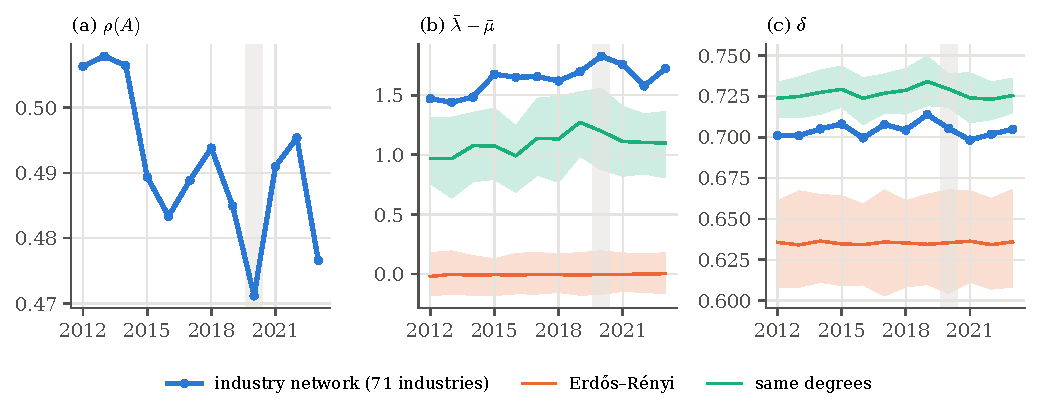
\includegraphics[width=\linewidth]{figures/fig-years.pdf}
\caption{Year by year, \YearFirst--\YearLast, for the \NSummary{}-industry
tables: (a) the spectral radius $\rho(A)$; (b) the gap $\bar\lambda-\bar\mu$
and (c) $\delta$, at the threshold matching the density of $H(2,20)$, with the
central $95\%$ ranges of the two random benchmarks. The year 2020 is shaded.}
\label{fig:years}
\end{figure}

\paragraph{Summary.} On these tables, supply chains are short: half of all
requirements are direct purchases, and the average chain is about two steps
long, with longer chains decaying at the rate $\rho(A)$. As a graph, the
network is dominated by a few service industries that supply most other
industries.
Even so, whether two industries trade directly predicts how many trading
partners they share more strongly than the unequal degrees alone would
produce. What separates the network from strong regularity is variation: the
number of shared partners varies greatly from one pair to the next, which
accounts for most of $\delta$. These are statements about the US input--output
tables over 2012--2023, not general facts about supply chains.

% ---------------------------------------------------------------------
\subsection{Limitations}
\label{subsec:supply-limits}

An industry aggregates many firms, so an edge between two industries does not
mean that any particular firms trade; firm-level supplier networks are not
publicly available. The tables record total requirements, including inputs
that were imported, so $A$ describes the technology of US production rather
than purely domestic supply chains. Thresholding discards both the size of
each requirement and its direction; we report a sweep of thresholds for the
first reason, and the directed matrix $A$ itself is used in
Section~\ref{subsec:walks}. Restricting to the $400$ largest industries treats
the two smallest as outside suppliers; no industry buys more than
\DroppedShare{} cents of inputs from them per dollar of its output. Finally, the benchmarks are deliberately extreme: a
network that sits between them is neither perfectly uniform nor random, which
is informative but is not a model of how supply chains form.
